\chapter{Theory} \label{chap:theory}

This chapter describes the theory behind blending and deblending. First the detail hiding operator notation is explained. This notation is used to describe the forward model of seismic data. By introducing the blending operator the forward model is extended to the blended case. Next, the deblending method of \citet{Mahdad-Deblending-Method} is discussed to illustrate the concepts on which this thesis is based. At the end of the chapter the blending operator is analyzed in greater detail, and the extension to 3D is discussed.

\section{The Forward Model of Blending} \label{sec:Ch-Theory-Operator}
%The detail hiding operator notation was introduced by \citet{Berkhout1982}, and later on it was extended for blended data. 

\subsection{Conventional Seismic Data}
In the detail hiding operator notation \citep{Berkhout1982} the recorded signal is considered discrete in terms of time $t$, receiver position $x_r$, and source position $x_s$. Thus, the measurements can be organized in a cube, $\mathbf{p(t,x_r,x_s)}$ (see Figure \ref{fig:Ch-Theory-DataMatrix}). Each frequency slice of this new cube represents the data matrix, $\mathbf{P}$. 

In the data matrix, $\mathbf{P}$, each column corresponds to a monochromatic common shot gather, each row to a monochromatic common receiver gather, each diagonal to a monochromatic common offset gather, and each anti-diagonal to a monochromatic common midpoint gather. These properties are summarized in Figure \ref{fig:Ch-Theory-DataMatrixMahdad}. 

\begin{figure}
    \centering
	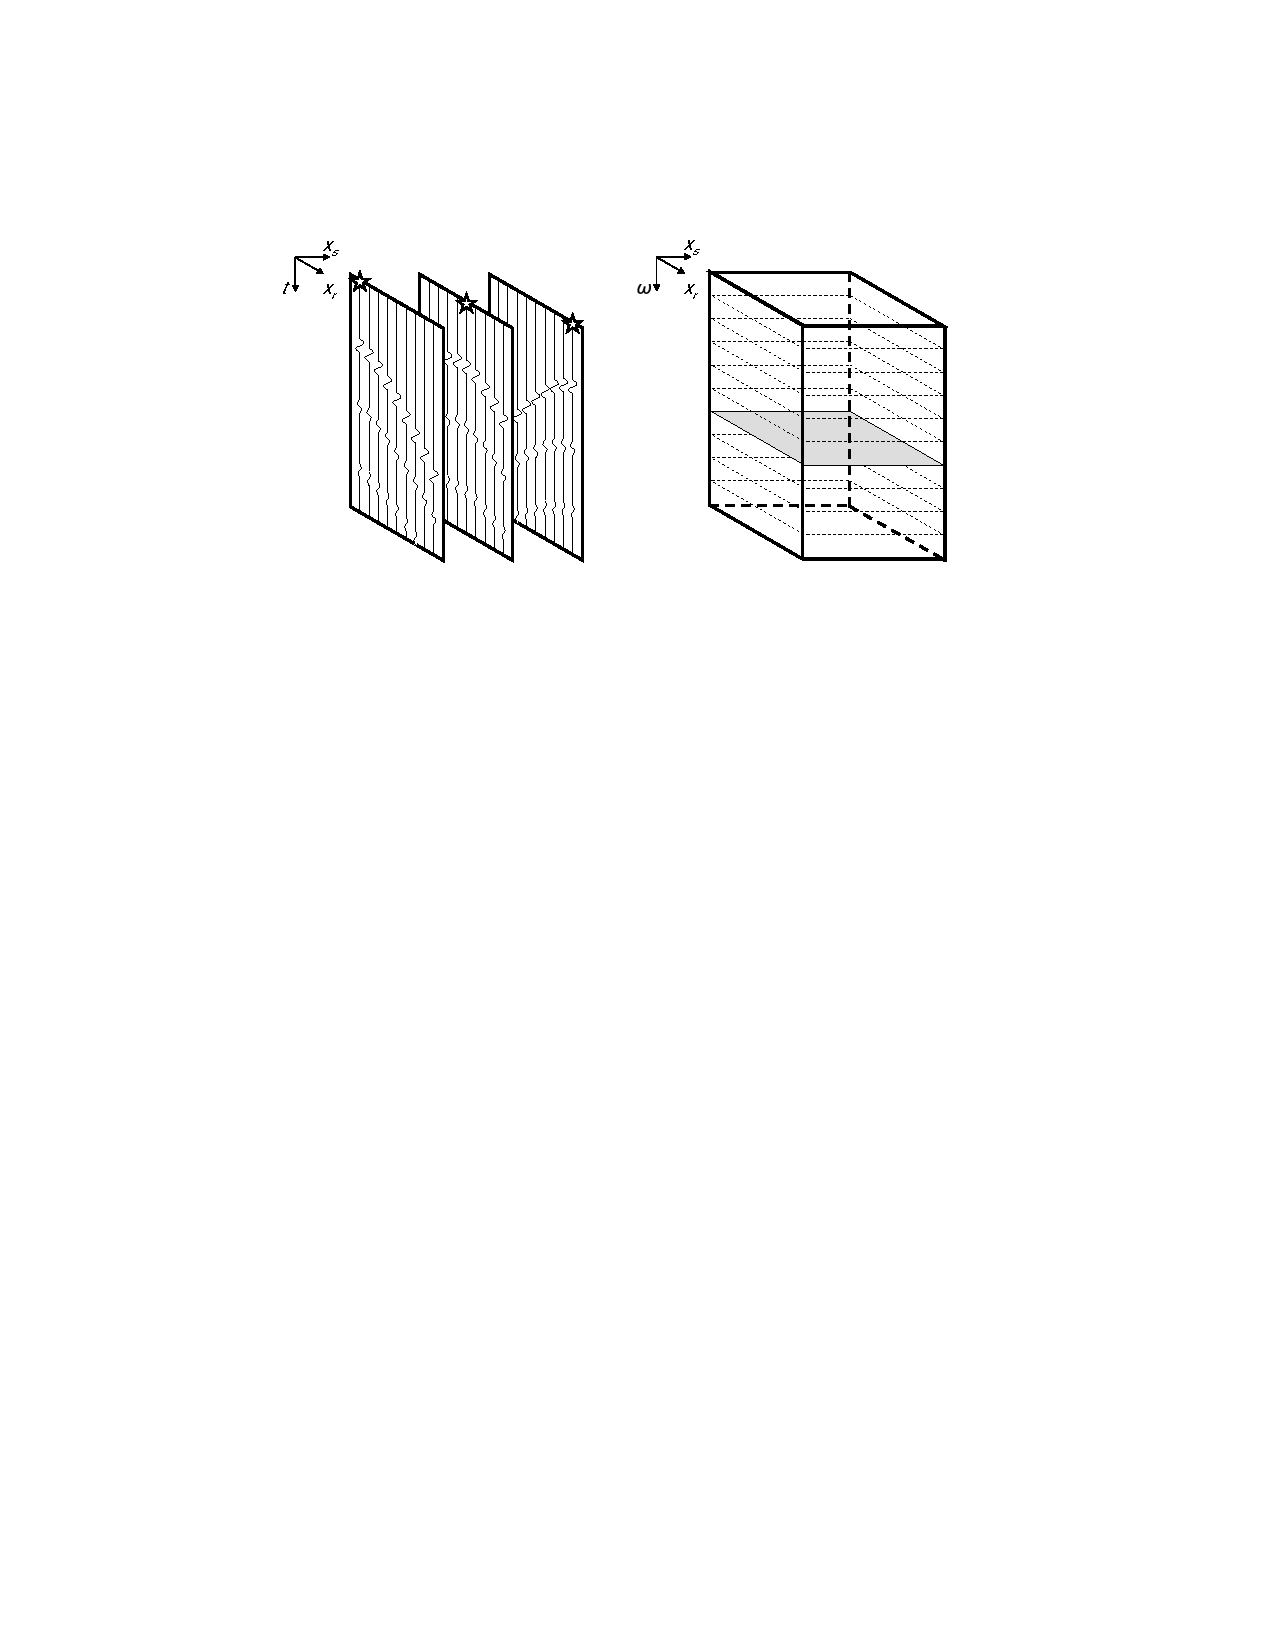
\includegraphics{Plots/P-Groenestijn_2010}
	\caption{Illustration of the data matrix, $\mathbf{P}$, by \citet{Groenestijn_2010}. \textit{Left:} The signal generated at the source position, $x_s$, is measured at receiver position, $x_r$, as a function of time, $t$. Thus, the discretized data is saved in a cube, $\mathbf{p(t,x_r,x_s)}$. \textit{Right:} The cube on the right equals the left cube after a Fourier transform with respect to time. Each frequency slice of the right cube represents the data matrix, $\mathbf{P}$.}
	\label{fig:Ch-Theory-DataMatrix}
\end{figure}


\begin{figure}
    \centering
	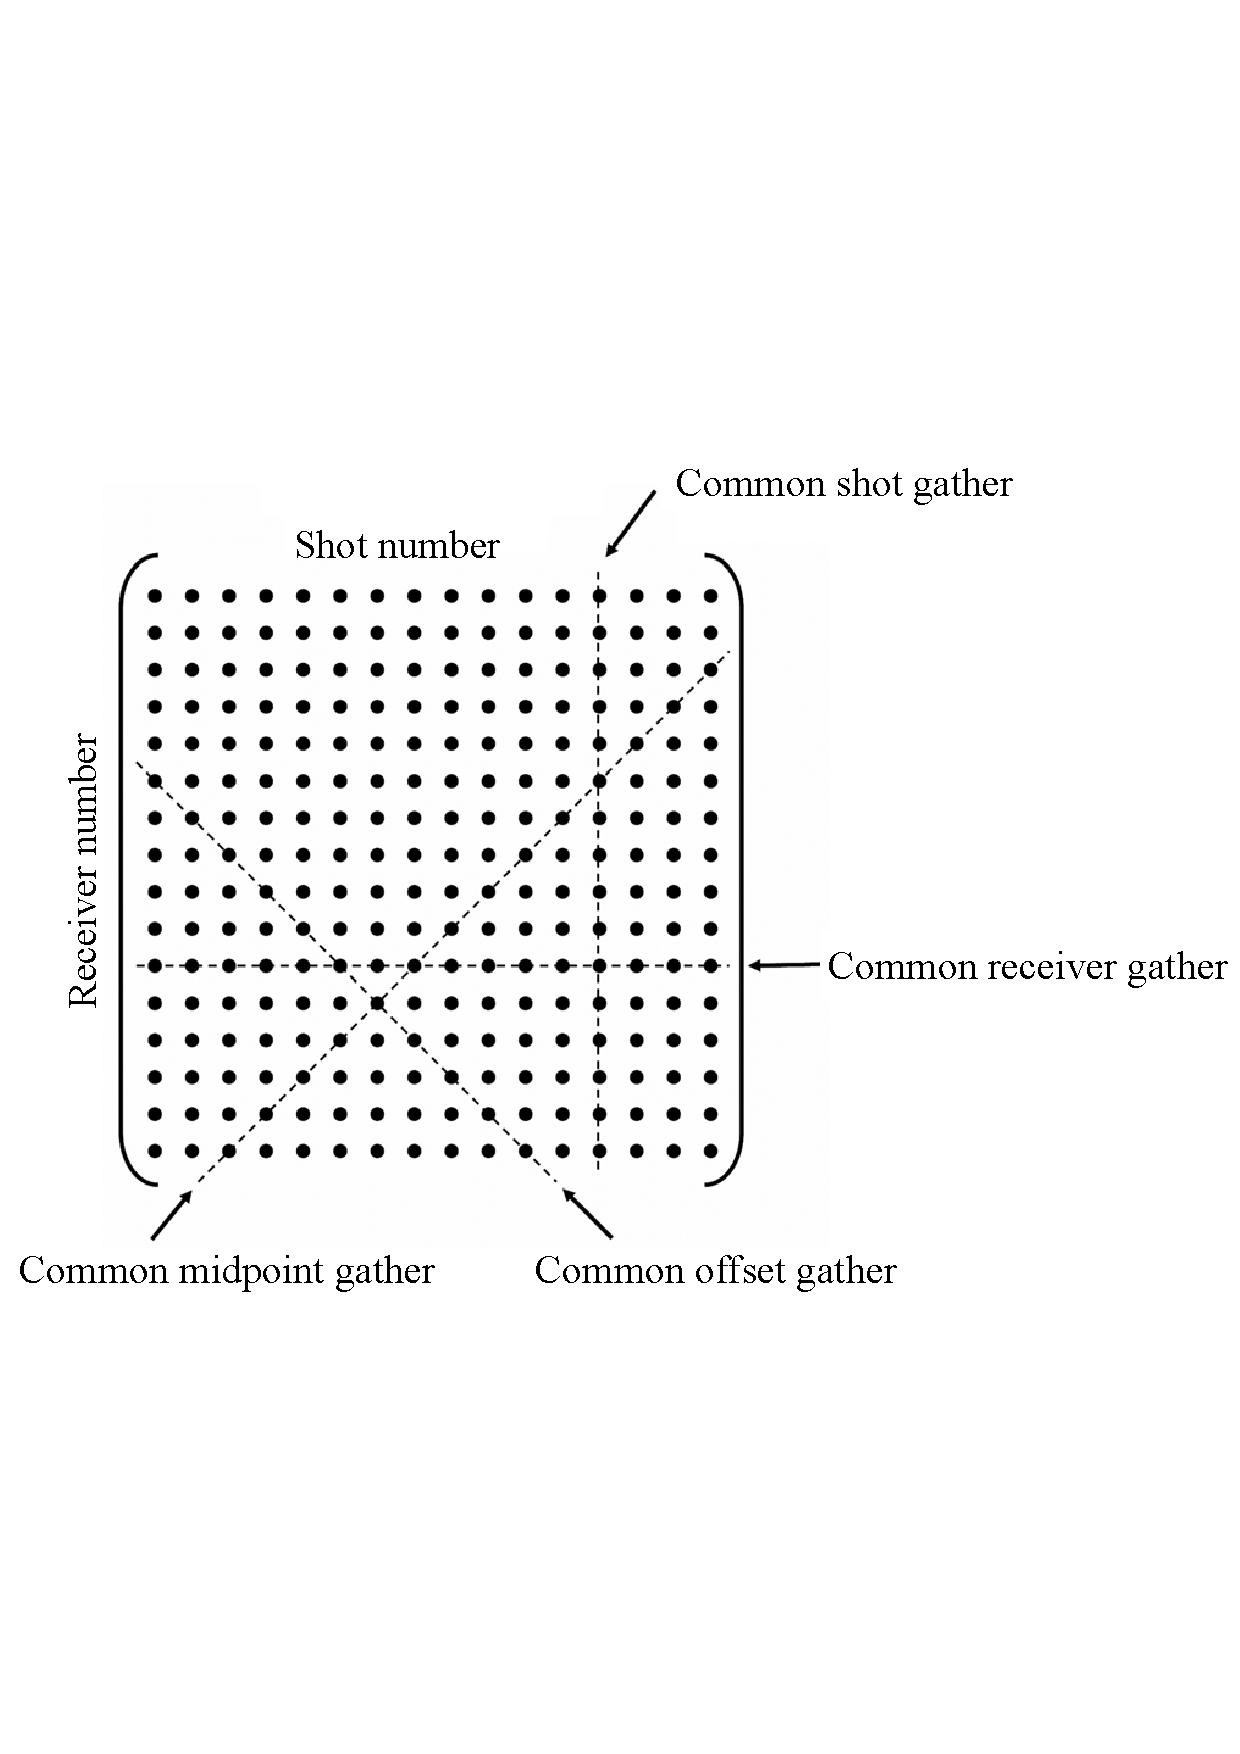
\includegraphics[width = 0.6\textwidth]{Plots/Mahdad-Data-Matrix-edited}
	\caption{Illustration of the data matrix, $\mathbf{P}$, by \cite{Mahdad-Deblending-Method}. The dotted lines indicate directions of common gathers.}
	\label{fig:Ch-Theory-DataMatrixMahdad}
\end{figure}

Based on the seismic forward model of \citet{Berkhout1982} the data matrix, $\mathbf{P}$, can be represented by a matrix multiplication of the source matrix, $\mathbf{S}$, the impulse response of the Earth, $\mathbf{X}$, and the receiver matrix, $\mathbf{D}$:

\begin{equation}
	\mathbf{P} = \mathbf{D \, X \, S}.
	\label{eq:Ch-Theory-DataRepresentation}
\end{equation}

In the source matrix, $\mathbf{S}$, each row and each column represent one source position (see Figure \ref{fig:Ch-Theory-BlendedSource}). Thus, $\mathbf{S}$ is a diagonal matrix. $\mathbf{S}$ captures one frequency component of the source signature. By applying a Fourier transform to all frequency components the source signature is obtained.

 The impulse response of the Earth, $\mathbf{X}$, describes how an impulse at the source location, $x_s$, is transformed in the Earth into the signal at the receiver location, $x_r$.

$\mathbf{D}$ is the receiver matrix, which converts the seismic wavefield at the receiver location $x_r$ to the recorded signal.

In practice, one tries to retrieve the unknown Earth response, $\mathbf{X}$, from the data, $\mathbf{P}$, by removing $\mathbf{S}$ (designature) and $\mathbf{D}$ (receiver deghosting).

\subsection{Blended Seismic Data}

For blended acquisition the recorded events belonging to different sources overlap as shown in the shot gather in Figure \ref{fig:Ch-Theory-BlendedData}. 

\begin{figure}
	\centering
	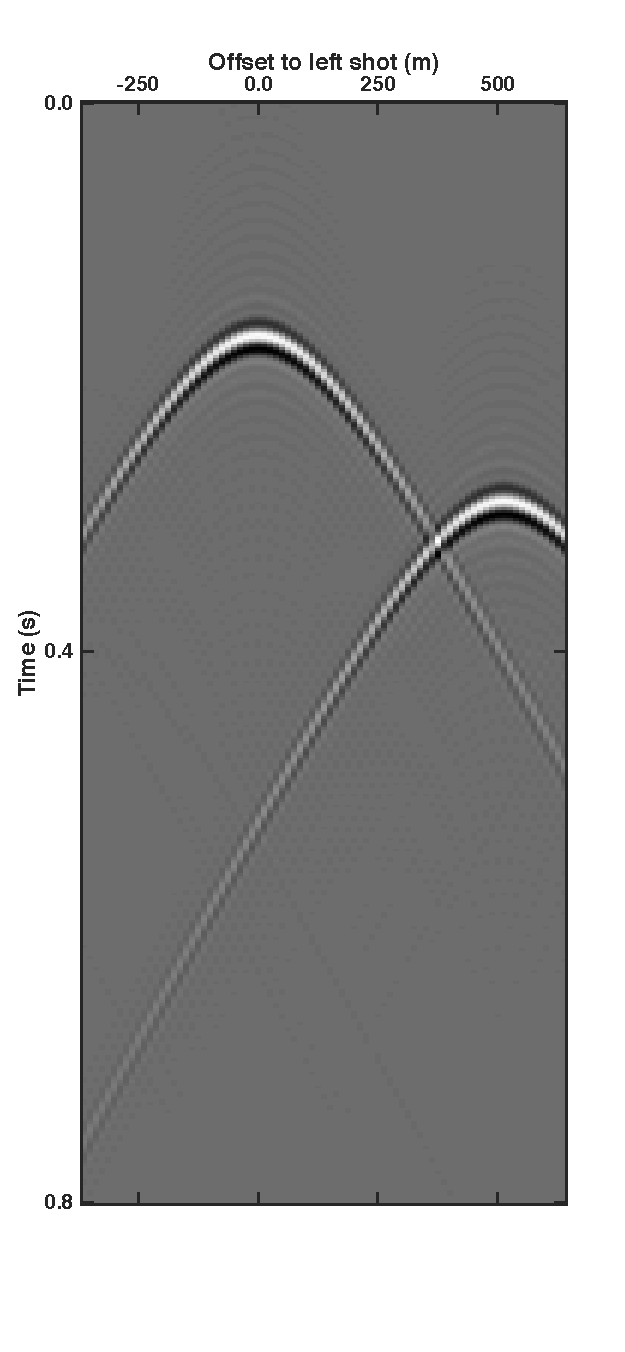
\includegraphics[width=0.25\textwidth]{Plots/Mahdad/30iter/BlendedCSG_sh1-edit_copy}
	\caption{Common shot gather of two blended shots with a time delay of about \SI{120}{\milli\second}.}
	\label{fig:Ch-Theory-BlendedData}
\end{figure}

This can be captured in the forward model by introducing a blending matrix, $\mathbf{\Gamma}$, which transforms the source matrix, $\mathbf{S}$, into a blended source matrix, $\mathbf{S_{bl}}$,

\begin{equation}
	\mathbf{S_{bl}} = \mathbf{S \, \Gamma}.
	\label{eq:Ch-Theory-BlendedSource}
\end{equation}

 Each row of $\mathbf{\Gamma}$ represents one source, and each column of $\mathbf{\Gamma}$ represents one experiment (see Figure \ref{fig:Ch-Theory-BlendedSource}). 
 
 The blending matrix captures the physics of a blended acquisition as follows: An element $\gamma_{ij}$ of the blending matrix relates a source $i$ to an experiment $j$. Within the experiment $j$ the source $i$ has a relative amplitude $A_{ij}$ and a relative time delay $t_{ij}$ with respect to the first source fired in the $j^{th}$ experiment. If the source $i$ is not fired in the $j^{th}$ experiment the amplitude $A_{ij}$ is zero. Based on these considerations the element $\gamma_{ij}$ is described with an amplitude term $A_{ij}$ and a phase term $\mathrm{e}^{-j \omega \Delta t_{ij}}$; 

\begin{equation}
	\gamma_{ij} =  A_{ij} \mathrm{e}^{-j \omega \Delta t_{ij}}.
	\label{eq:Ch-Theory-BlendingElement}
\end{equation} 

Thus, the blending matrix selects specific sources from the source matrix and superimposes as visualized in Figure \ref{fig:Ch-Theory-BlendedSource}. From Figure \ref{fig:Ch-Theory-BlendedSource} it also becomes clear that both the blending matrix, $\mathbf{\Gamma}$, and the blended source matrix, $\mathbf{S_{bl}}$, have more rows than columns. 

\begin{figure}
	
	\centering
	\begin{subfigure}[t]{0.6\textwidth}	
	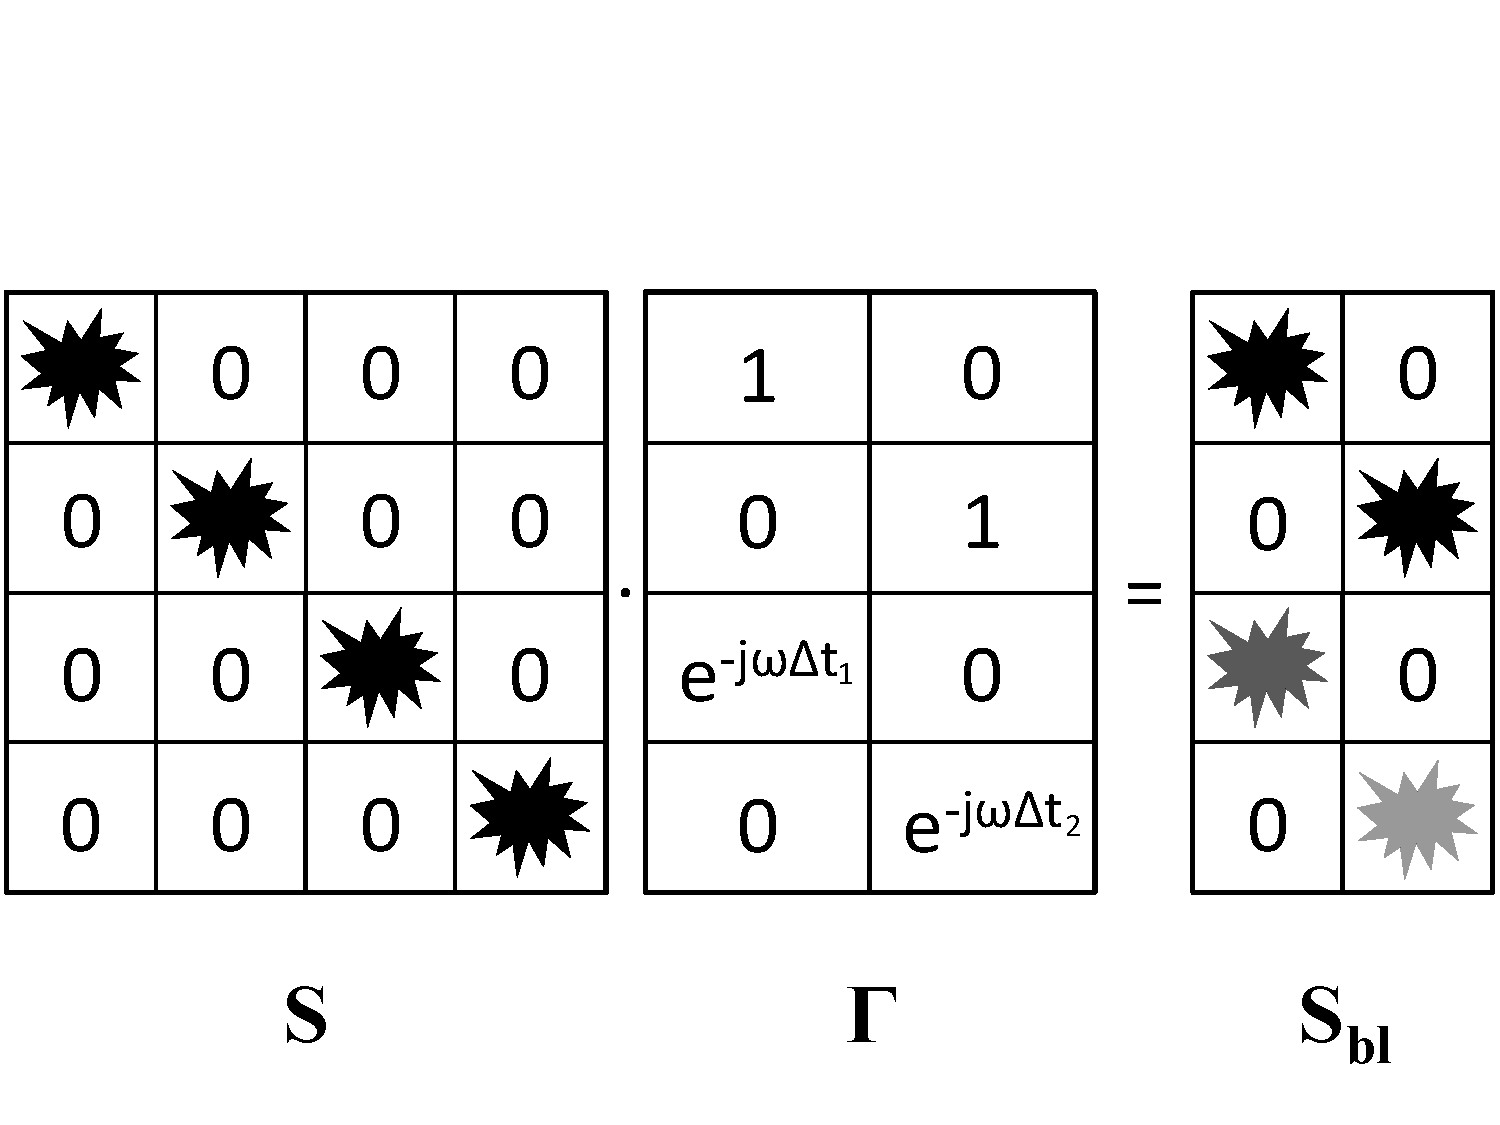
\includegraphics[width=\textwidth]{Plots/Blended-Source-edit2}
	\caption{}
	\label{fig:Ch-Theory-BlendedSource-Matrices}
	\end{subfigure}
	\par\bigskip
	\begin{subfigure}[t]{\textwidth}
	\centering
	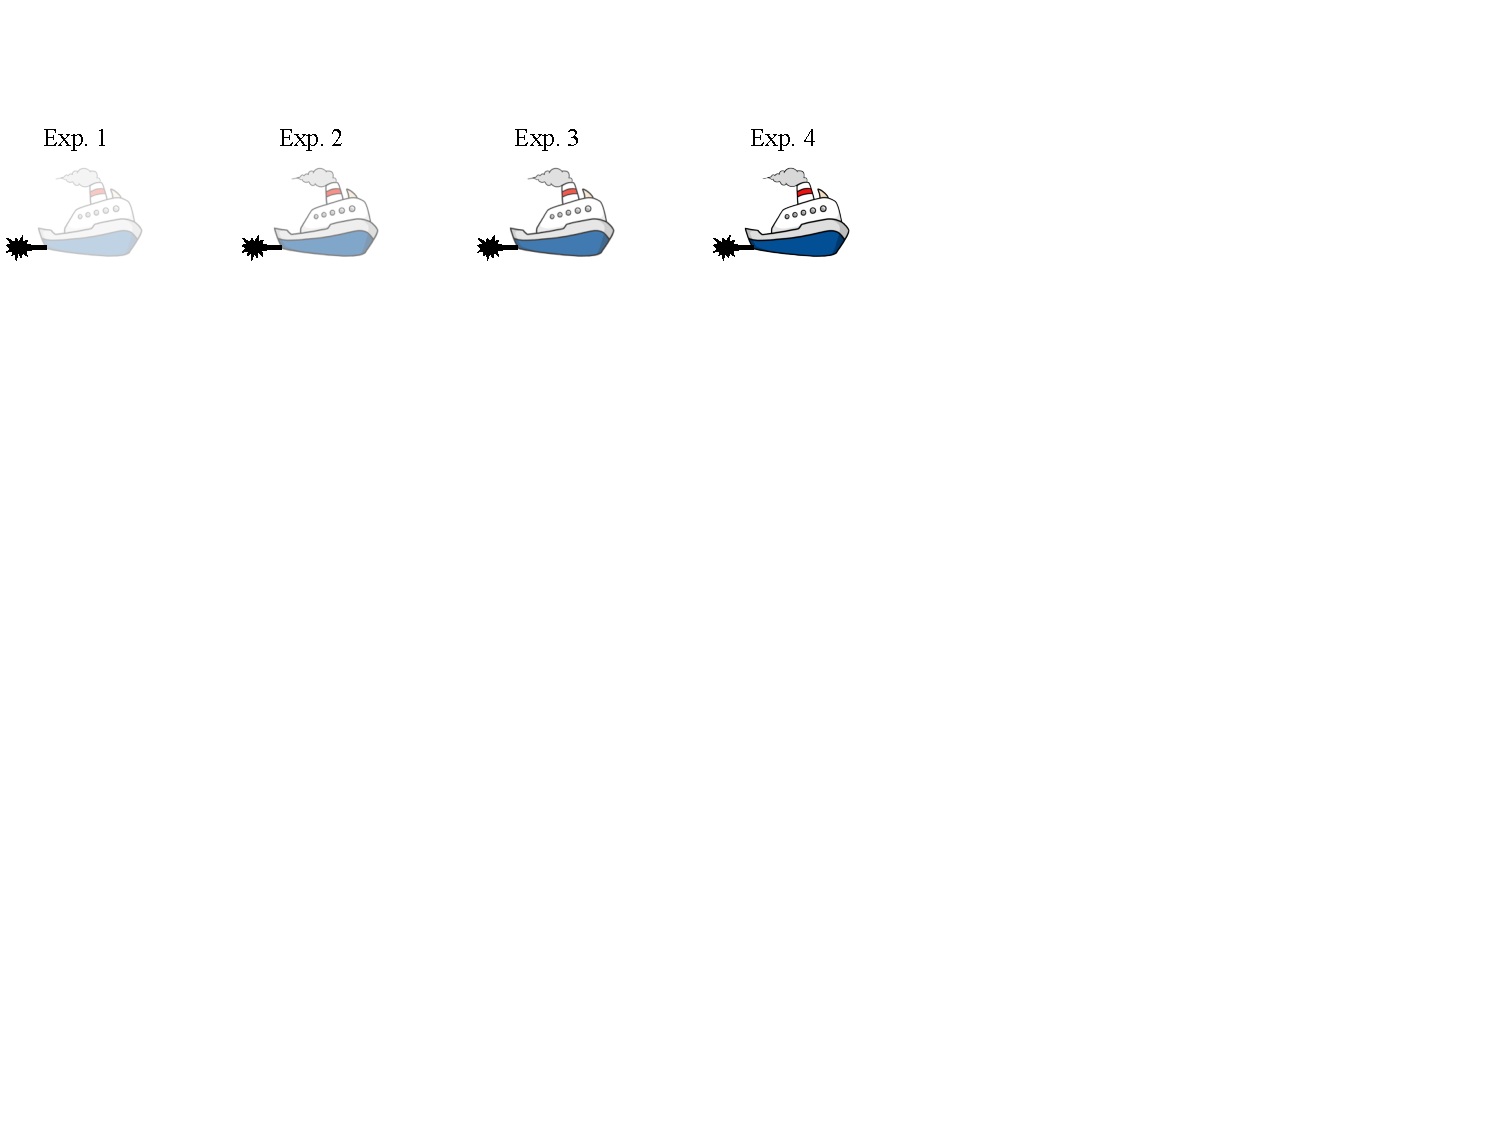
\includegraphics[width=0.5\textwidth]{Plots/Blended-Source-Conventional}
	\caption{}
	\label{fig:Ch-Theory-BlendedSource-Conventional}
	\end{subfigure}
	\par\bigskip
	\begin{subfigure}[t]{\textwidth}
	\centering
	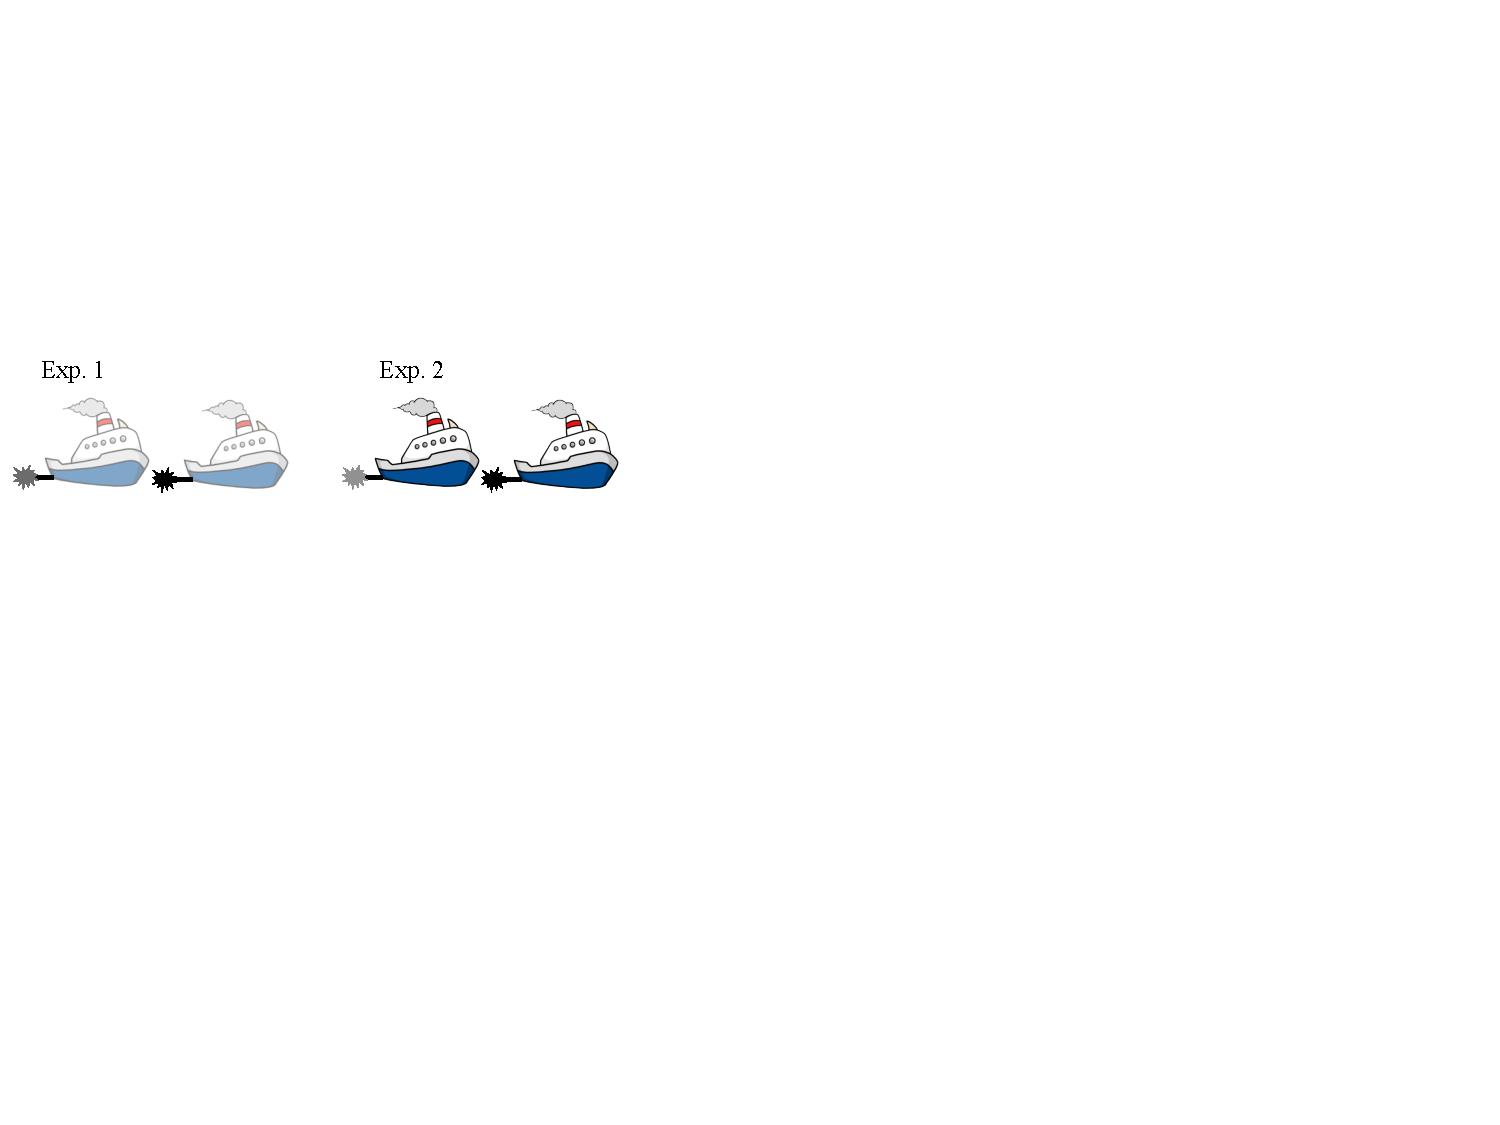
\includegraphics[width=0.36\textwidth]{Plots/Blended-Source-New}
	\caption{}
	\label{fig:Ch-Theory-BlendedSource-Blended}
	\end{subfigure}
    % RATIO of the boat images 294 : 410
	
	\caption{(a) A conventional source matrix, $\mathbf{S}$, is transformed to a blended source matrix, $\mathbf{S_{bl}}$, by applying the blending matrix, $\mathbf{\Gamma}$. Each star represents a source, and the gray scale of the stars represents the relative firing time. (b) Illustration of conventional acquisition with one vessel and the source matrix $\mathbf{S}$. (c) Illustration of blended acquisition with two vessels and the source matrix $\mathbf{S_{bl}}$. The experiment number is indicated on top of each drawing.}
	\label{fig:Ch-Theory-BlendedSource}
	
\end{figure}

In the case of source blending the receiver matrix, $\mathbf{D}$, is not influenced by blending. And of course, the Earth impulse response, $\mathbf{X}$, is independent of the acquisition design. Hence, the blended data can be written as;

\begin{equation}
	\mathbf{P_{bl}} = \mathbf{D} \, \mathbf{X} \, \mathbf{S_{bl}} = \mathbf{D} \, \mathbf{X} \, \mathbf{S} \, \mathbf{\Gamma} = \mathbf{P \, \Gamma}.
	\label{eq:Ch-Theory-BlendedData}
\end{equation}

Note that the blended data matrix, $\mathbf{P_{bl}}$, has less columns, i.e. less experiments, than the unblended data matrix, $\mathbf{P}$.



\section{Deblending} \label{sec:MahdadMethod}

The deblending method in this thesis builds on the method of \citet{Mahdad-Deblending-Method}. Therefore, the method of \citet{Mahdad-Deblending-Method} is described in detail. In section \ref{sec:MahdadMethod3d} it will be extended to 3D.


The basic workflow of the method of \citet{Mahdad-Deblending-Method} is summarized in Figure \ref{fig:Ch-Theory-FlowChart} and will be explained step by step in the following subsections. 

\begin{figure}
	\centering
	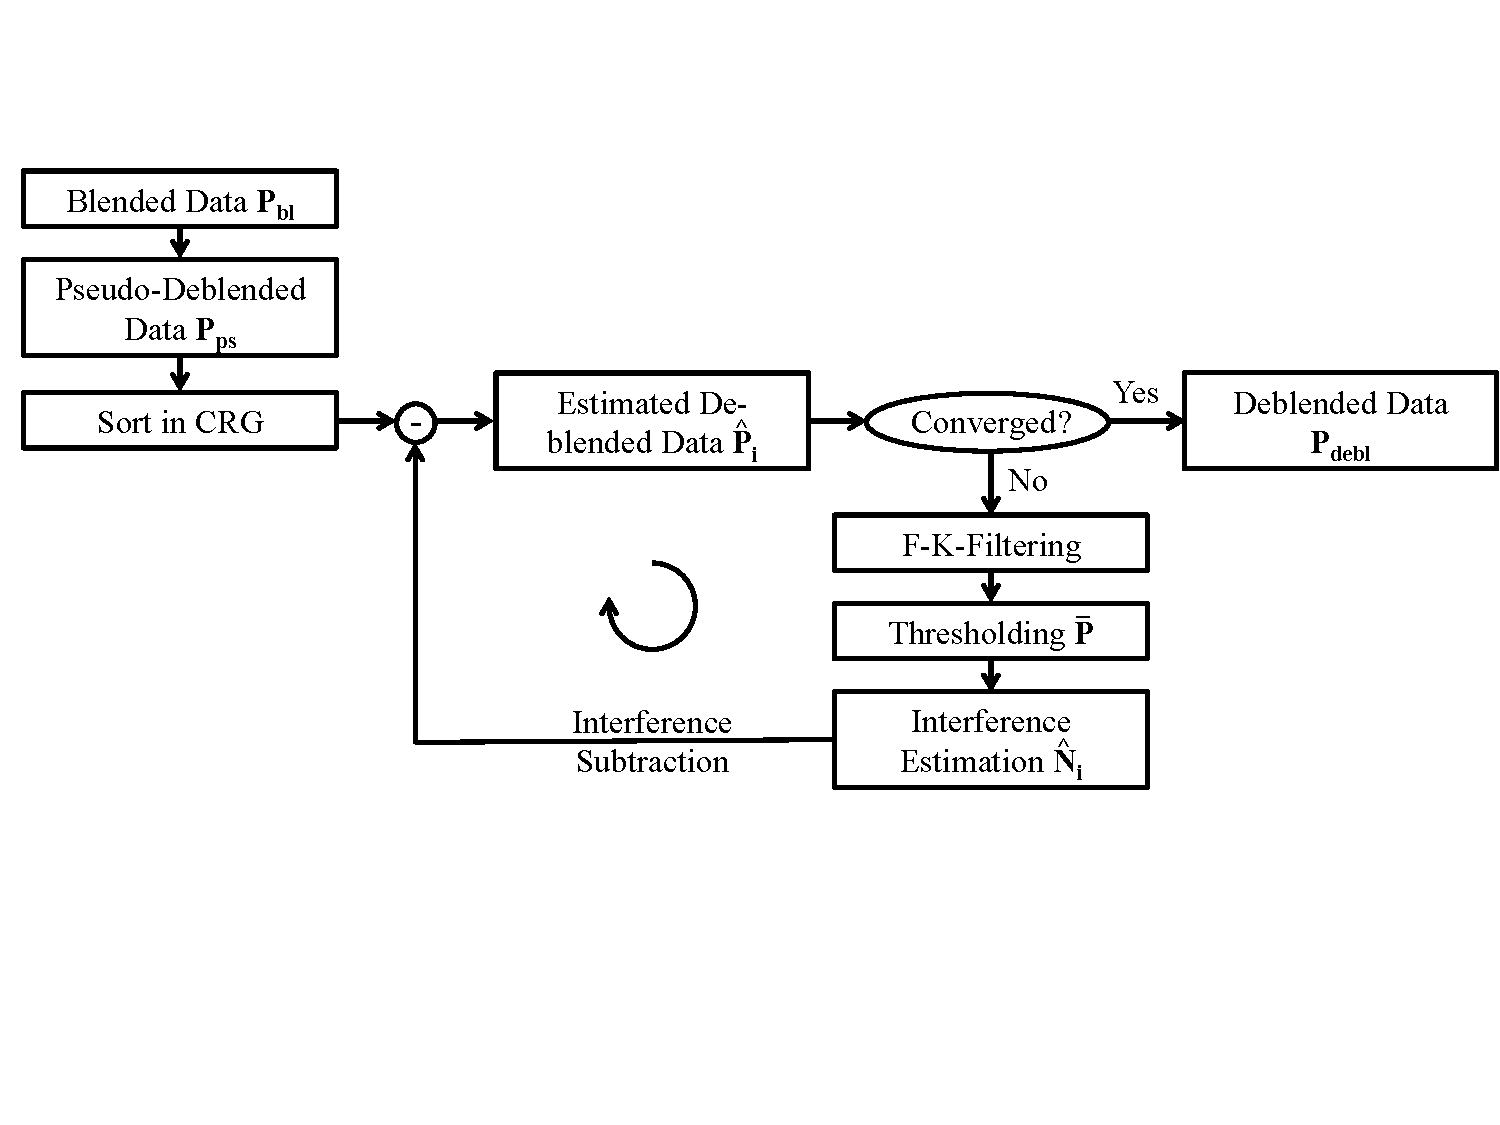
\includegraphics[width=0.8\textwidth]{Plots/Mahdad-FlowChart-v3}
	\caption{Pseudo-deblending provides a first estimate of the unblended data. The blended sources are incoherent in the common receiver domain. This incoherent blending noise is attenuated with f-k-filtering and thresholding. Next, the source interference is estimated and subtracted from the pseudo-deblended data. The deblended data is achieved when the data estimation converges.}
	\label{fig:Ch-Theory-FlowChart}
\end{figure}

\subsection{Pseudo-Deblending}

Unfortunately, the inverse problem of equation \ref{eq:Ch-Theory-BlendedData} is underdetermined, which means that there is not a unique solution for the unblended data, $\mathbf{P}$. Thus, additional constraints are required to deblend the data, which are sparsity of the signal in the $x$-$t$-domain and coherency of the signal in the $f$-$k$-domain. 

The first guess of the unblended data matrix, $\mathbf{P}$, is estimated via pseudo-deblending;

\begin{equation}
	\mathbf{P_{ps}} = \mathbf{P_{bl}} \, \mathbf{\Gamma^H}.
	\label{eq:Ch-Theory-PseudoDeblended}
\end{equation}

Pseudo-deblending copies the blended data to the locations of all shots present in the blended shot and shifts it  upward to compensate for the time delay of the blended source. For example, Figure \ref{fig:Ch-Theory-PseudoDeblendedCSG} shows the pseudo-deblended shot gather of the blended data in Figure \ref{fig:Ch-Theory-BlendedData}.


\subsection{Common Receiver Gather}
By transforming the data to another domain, e.g. to the common receiver domain, the interfering sources become incoherent and are visible as spiky noise (see Figure \ref{fig:Ch-Theory-PseudoDeblendedCRG}). Therefore, the interfering sources can be attenuated with a noise filter. The noise generated by the interfering sources is called blending noise. 
\todo[inline]{Considering the 1/b factor, the interfering source creates blending noise and scales the amplitude of the shot of interest. So, is it correct to set blending noise and interfering source equal?}

\begin{figure}
	\centering
	\begin{subfigure}[t]{0.25\textwidth}
		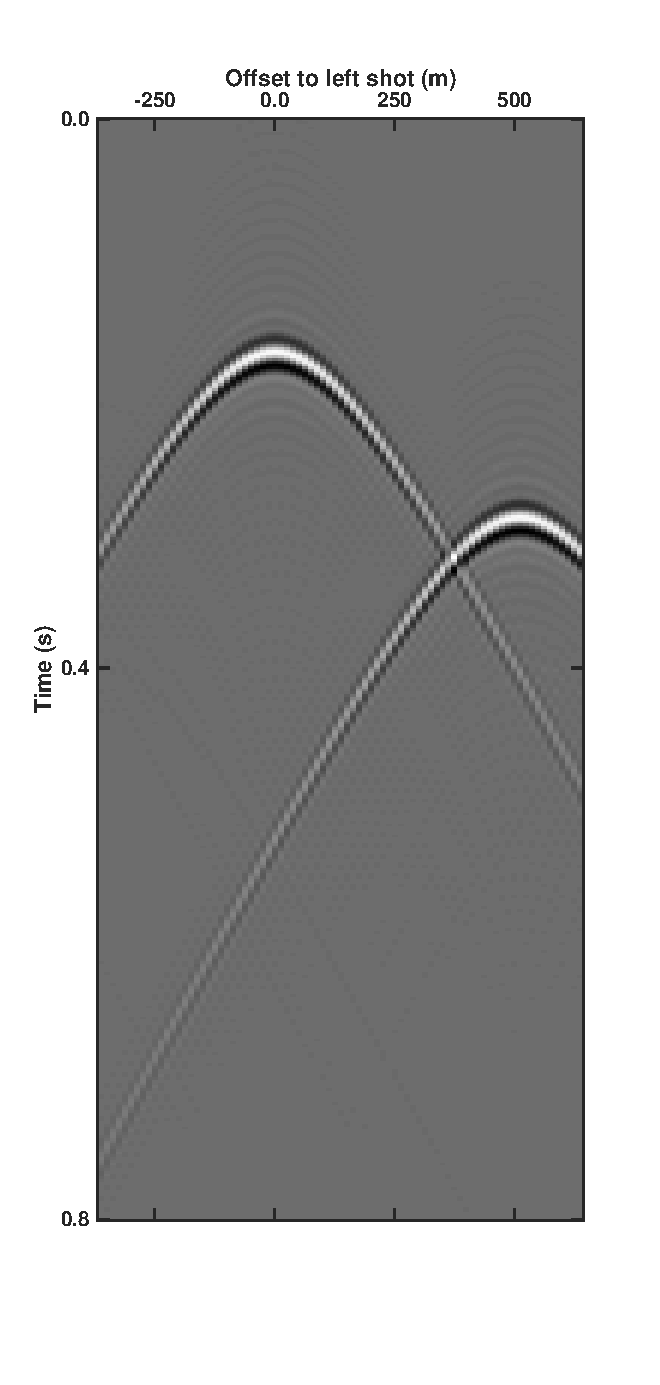
\includegraphics[width=\textwidth]{Plots/Mahdad/30iter/Pseudo-DeblendedCSG_sh1}	
		\caption{Common-shot-gather}
		\label{fig:Ch-Theory-PseudoDeblendedCSG}
	\end{subfigure}
	%
	\centering
	\begin{subfigure}[t]{0.25\textwidth}
		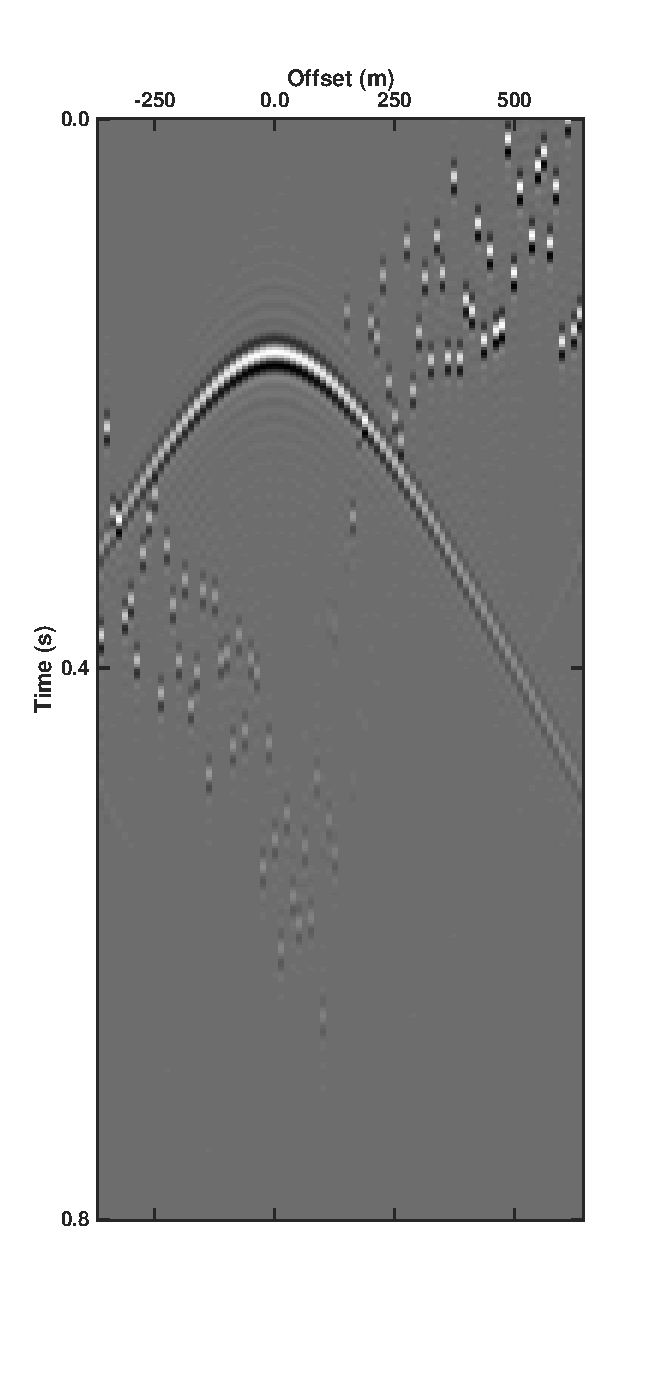
\includegraphics[width=\textwidth]{Plots/Mahdad/30iter/Pseudo-DeblendedCRG_rec30}	
		\caption{Common-receiver-gather}
		\label{fig:Ch-Theory-PseudoDeblendedCRG}
	\end{subfigure}
	\caption{Pseudo-deblended data, $\mathbf{P_{ps}}$, sorted in a common shot gather (left) and common receiver gather (right). The overlapping sources map in the pseudo-deblended shot gather as coherent events, while they map as incoherent spikes in the pseudo-deblended receiver gather.}
	\label{fig:Ch-Theory-PseudoDeblended}

\end{figure}

\subsection{Iterative Blending Noise Estimation}

Note that all the quantities which are estimated are indicated with a hat. The steps of the iterative blending noise estimation are demonstrated in Figure \ref{fig:Ch-Theory-IterativeDeblending}.

\subsubsection*{F-K-Filtering}
In an ideal case the blending noise, $\mathbf{N}$, which overlies the signal in the pseudo-deblended data would be calculated based on the unblended data,

\begin{equation}
	\mathbf{N} = \mathbf{P_{bl}} \, \mathbf{\Gamma^H} - \mathbf{P}.
	\label{eq:Ch-Theory-Noise}
\end{equation}

Obviously, in practice the unblended data is unknown and must be estimated by adding extra constraints. One of these constraints is coherency, i.e. by assuming the blending noise in Figure \ref{fig:Ch-Theory-PseudoDeblendedCRG} is incoherent it can be removed. For this purpose the data is transformed from the space time to the wavenumber frequency domain where the spiky noise spreads over all frequency and wavenumber components (see Figure \ref{fig:Ch-Theory-FKDeblended-NoFilter}, top). 


For a 2D $f$-$k$-spectrum the minimum (physical) velocity of the subsurface, $v_{min}$, determines the maximum unaliased wavenumber, $k_{max}$,  for a given frequency, $f$;

\begin{equation}
	k_{max} = \frac{f}{v_{min}}.
	\label{eq_Ch-Theory-MaxWavenmber}
\end{equation} 

For each frequency, $f$, wavenumbers above $k_{max}$ are removed which results in a 2D signal cone as depicted in Figure \ref{fig:Ch-Theory-FK-Mask}.

$f$-$k$-filtering removes the part of the blending noise, which maps outside of the signal cone. Thus, the amplitudes of the spiky noise in space time domain are attenuated (see Figure \ref{fig:Ch-Theory-FKFiltered}). 

Note that $f$-$k$-filtering can only reduce unaliased frequency components of the blending noise. In Figure \ref{fig:Ch-Theory-FK-Mask} the highest unaliased frequency is defined by the point where the white cone intersects with the frequency axis, i.e. at \SI{60}{\hertz}.

\begin{figure}
	\centering
	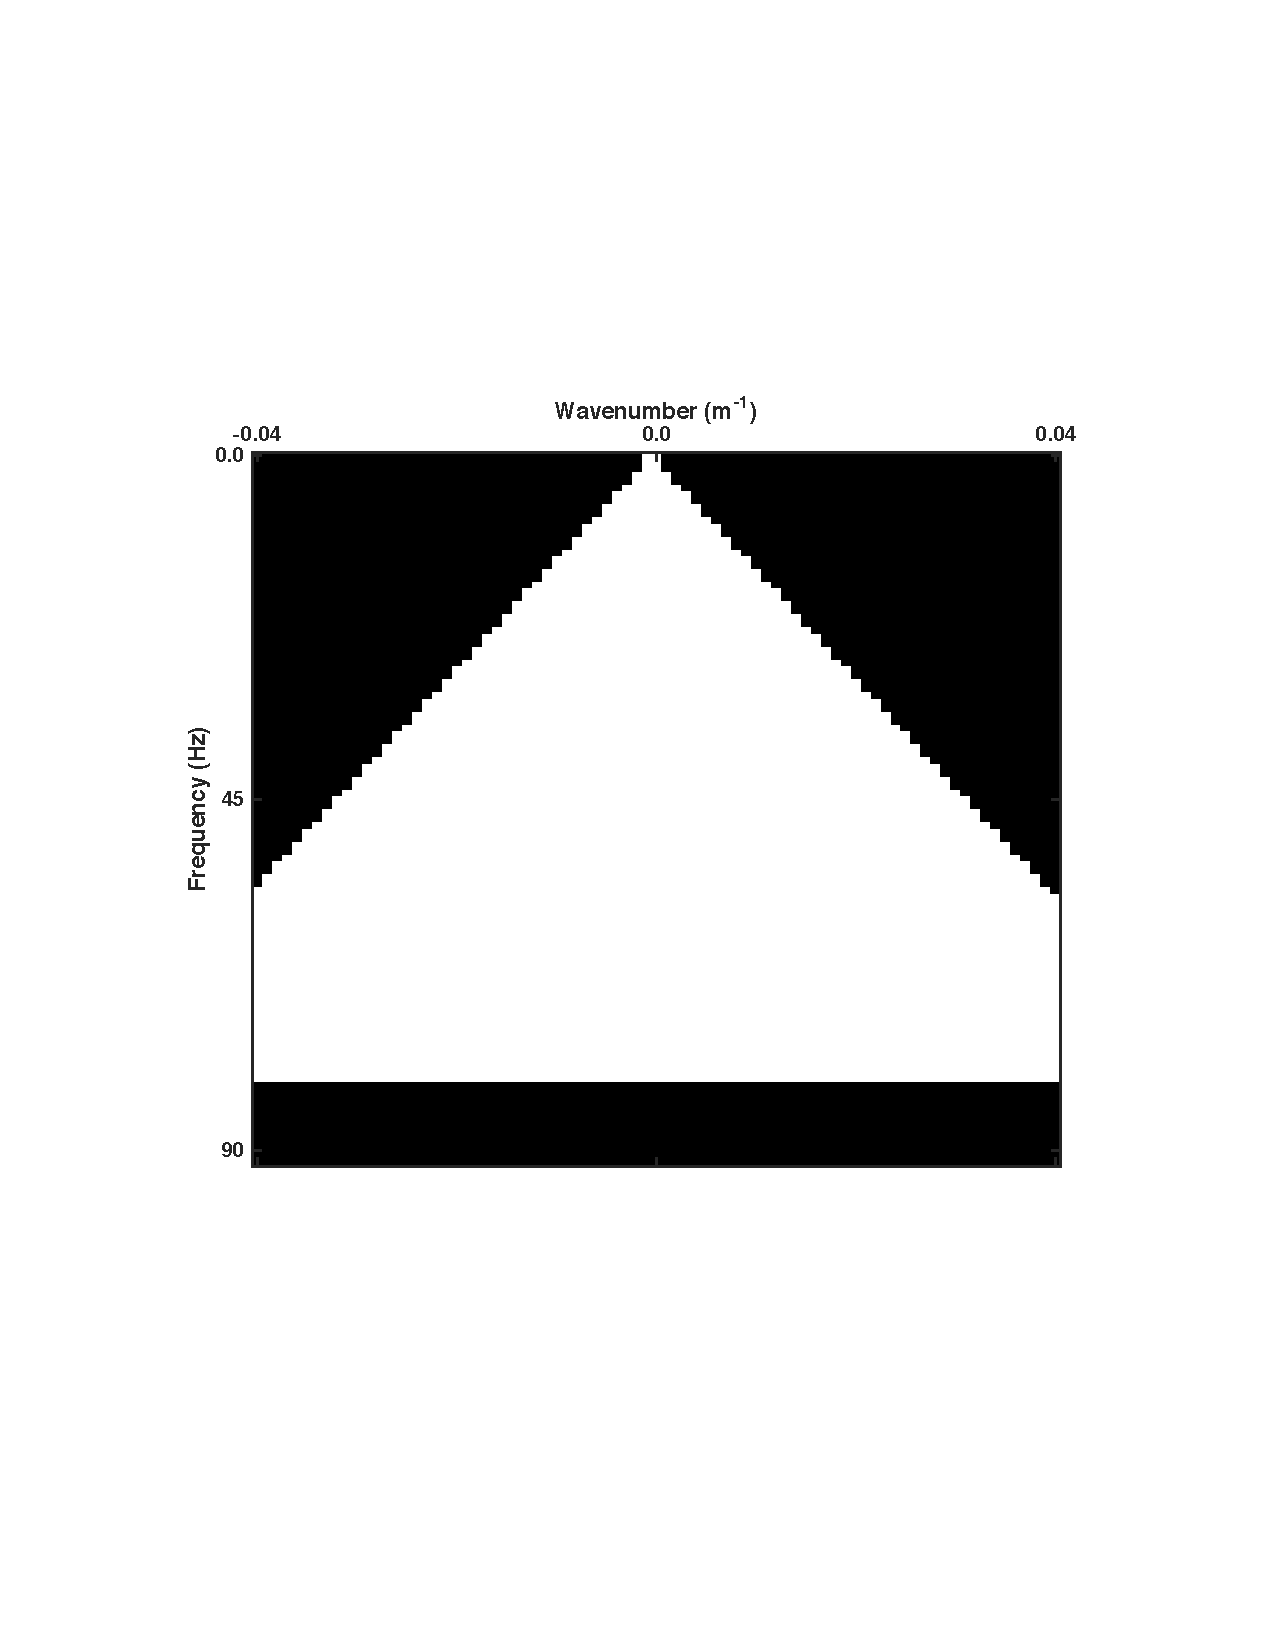
\includegraphics[width = 0.5\textwidth]{Plots/Mahdad/5iter/FK-MaskCRG_rec30}
	\caption{The $f$-$k$-mask is determined by the minimum signal velocity in the subsurface. The white area of the filter equals one, the black area equals zero. Thus, the filter removes data which is mapped outside of the white signal cone.}
	\label{fig:Ch-Theory-FK-Mask}
\end{figure}

 

\begin{figure}
	\centering
	\begin{subfigure}[t]{0.25\textwidth}
		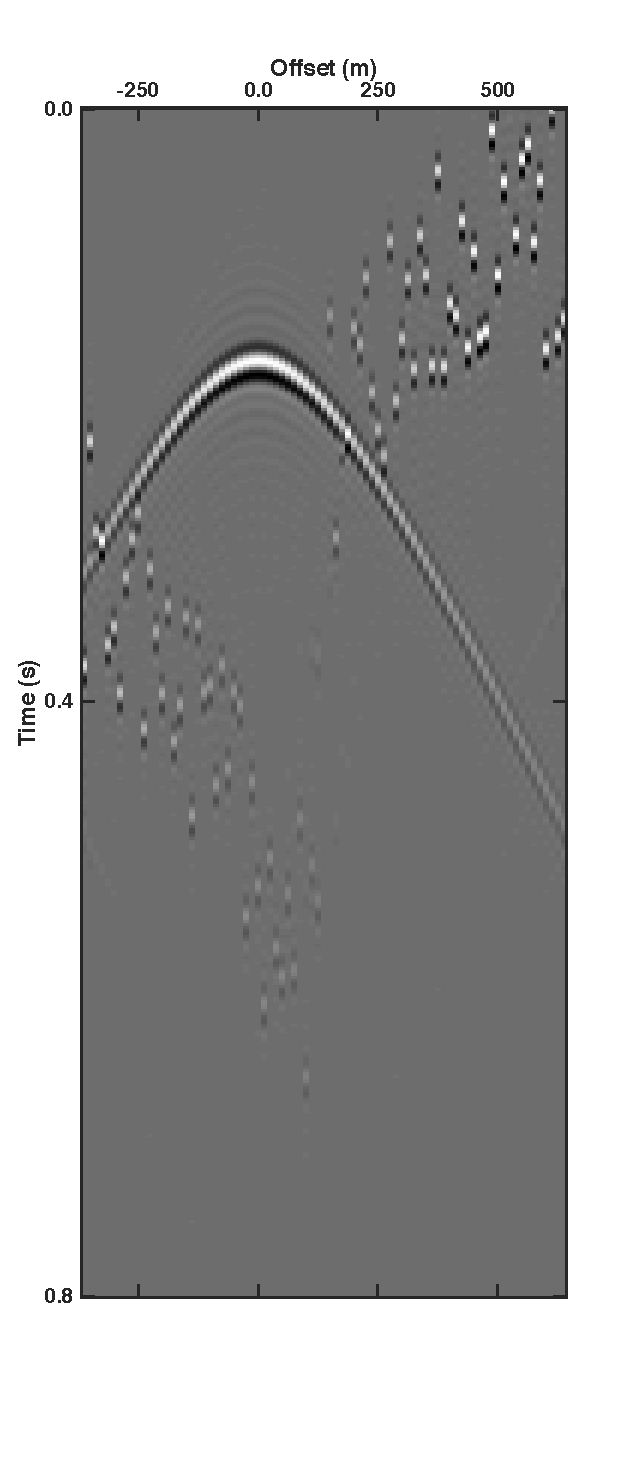
\includegraphics[width=\textwidth]{Plots/Mahdad/5iter/Pseudo-DeblendedCRG_rec30}	
		\caption{}
		\label{fig:Ch-Theory-PseudoDeblendedCRG5}
	\end{subfigure}
	%
	\centering
	\begin{subfigure}[t]{0.25\textwidth}
		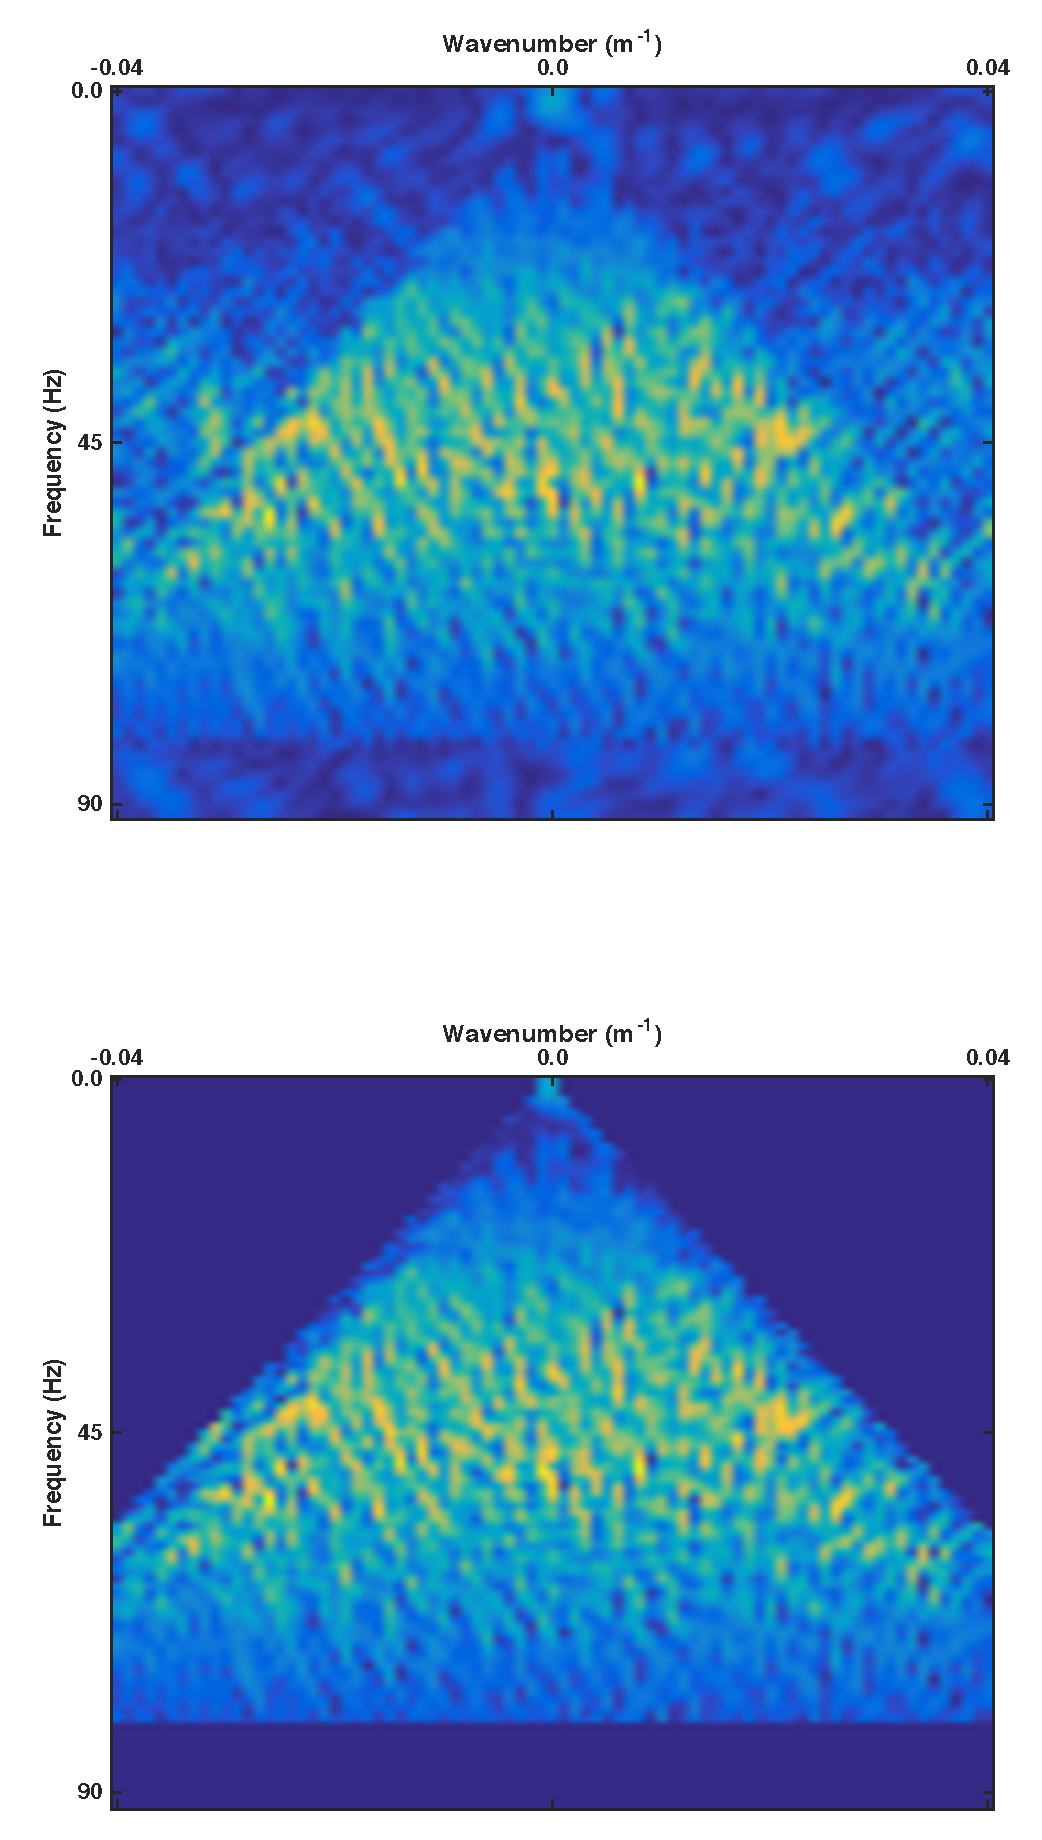
\includegraphics[width=\textwidth]{Plots/Mahdad/5iter/FK-Spectra}	
		\caption{}
		\label{fig:Ch-Theory-FKDeblended-NoFilter}
	\end{subfigure}
	%
	\begin{subfigure}[t]{0.25\textwidth}
		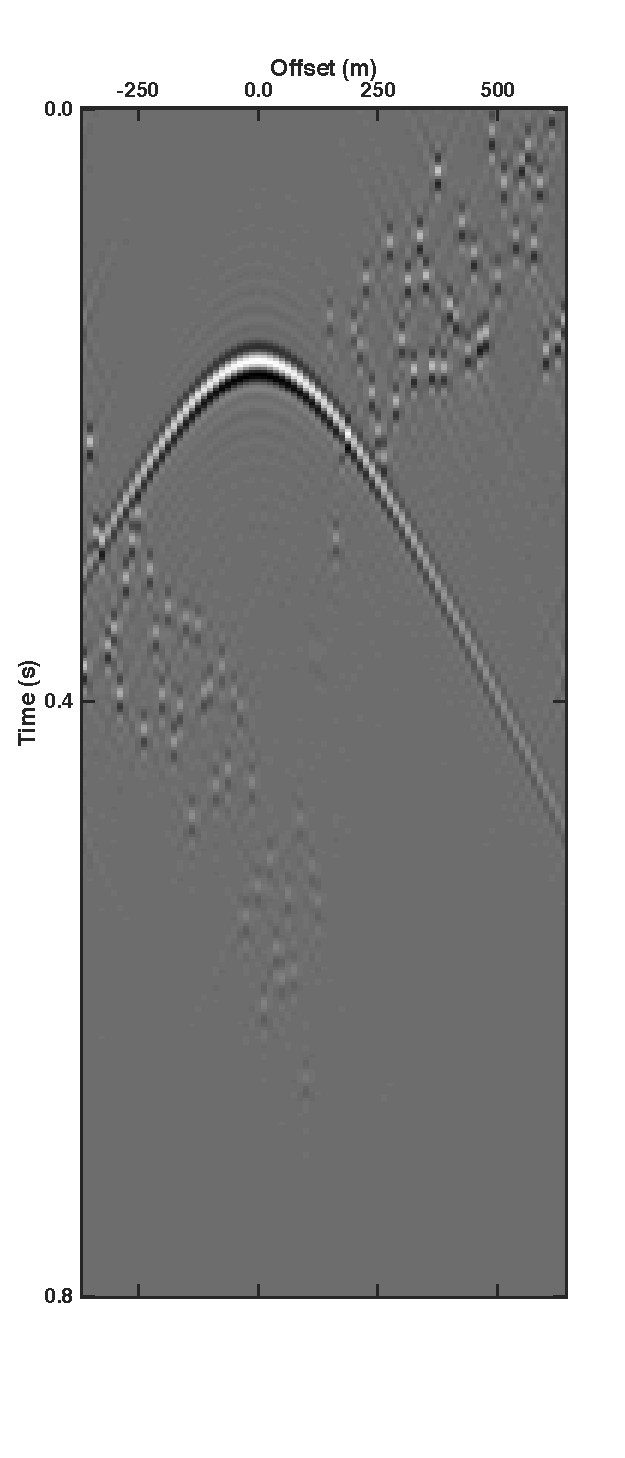
\includegraphics[width=\textwidth]{Plots/Mahdad/5iter/FkFilteredCRG_rec30}	
		\caption{}
		\label{fig:Ch-Theory-FKFiltered}
	\end{subfigure}
	%
	\begin{subfigure}[t]{0.25\textwidth}
		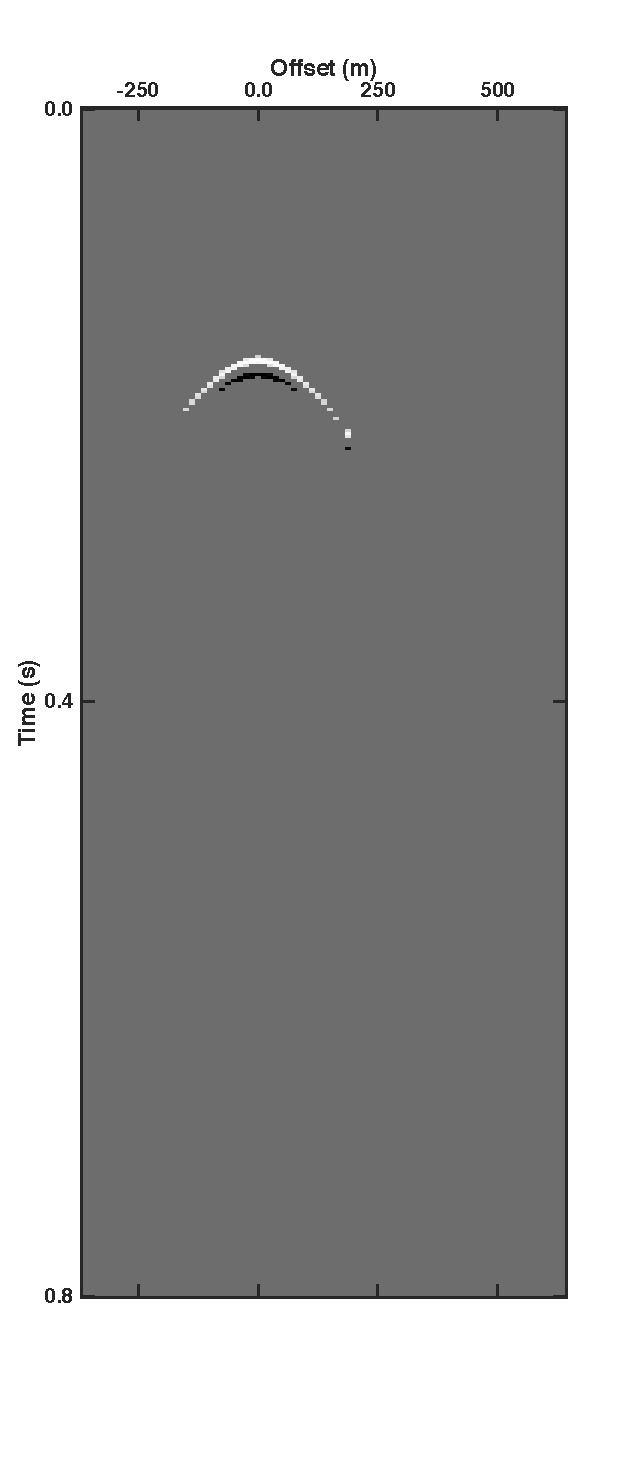
\includegraphics[width=\textwidth]{Plots/Mahdad/5iter/ThresholdCRG_rec30}	
		\caption{}
		\label{fig:Ch-Theory-Threshold}
	\end{subfigure}
	%
	\begin{subfigure}[t]{0.25\textwidth}
		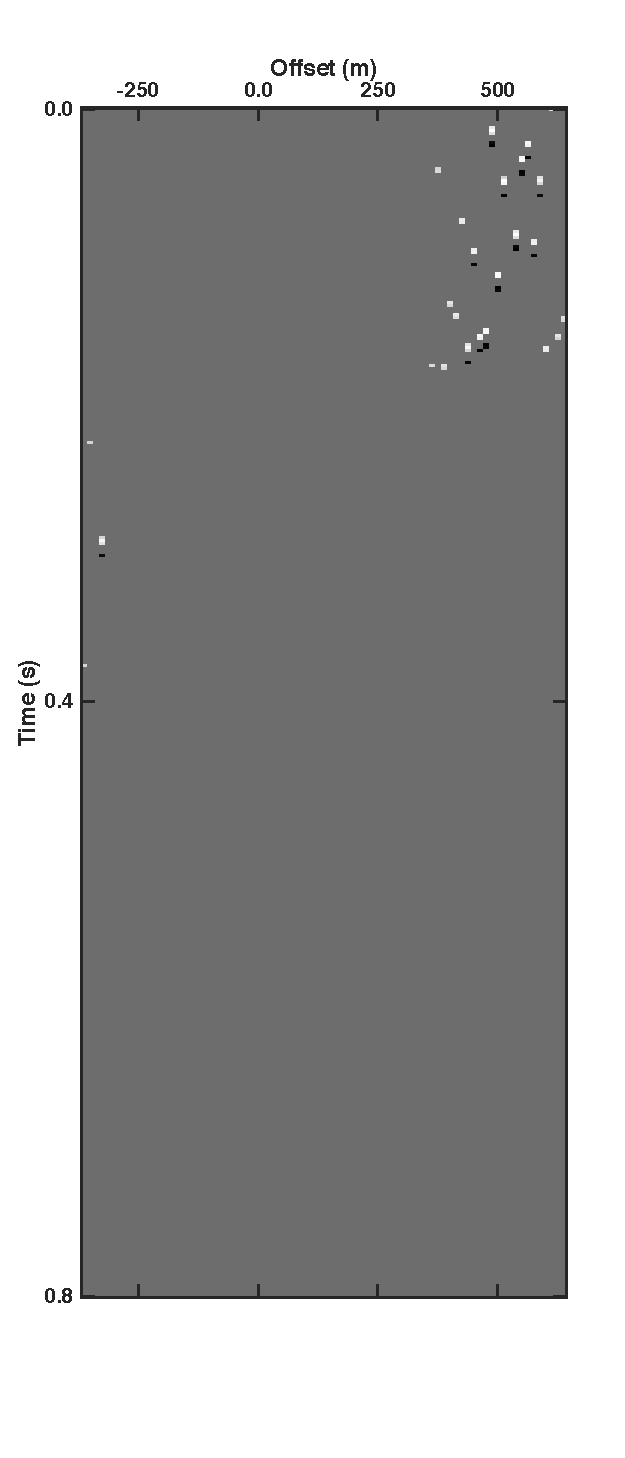
\includegraphics[width=\textwidth]{Plots/Mahdad/5iter/NoiseCRG_rec30}	
		\caption{}
		\label{fig:Ch-Theory-Noise}
	\end{subfigure}
	%
	\begin{subfigure}[t]{0.25\textwidth}
		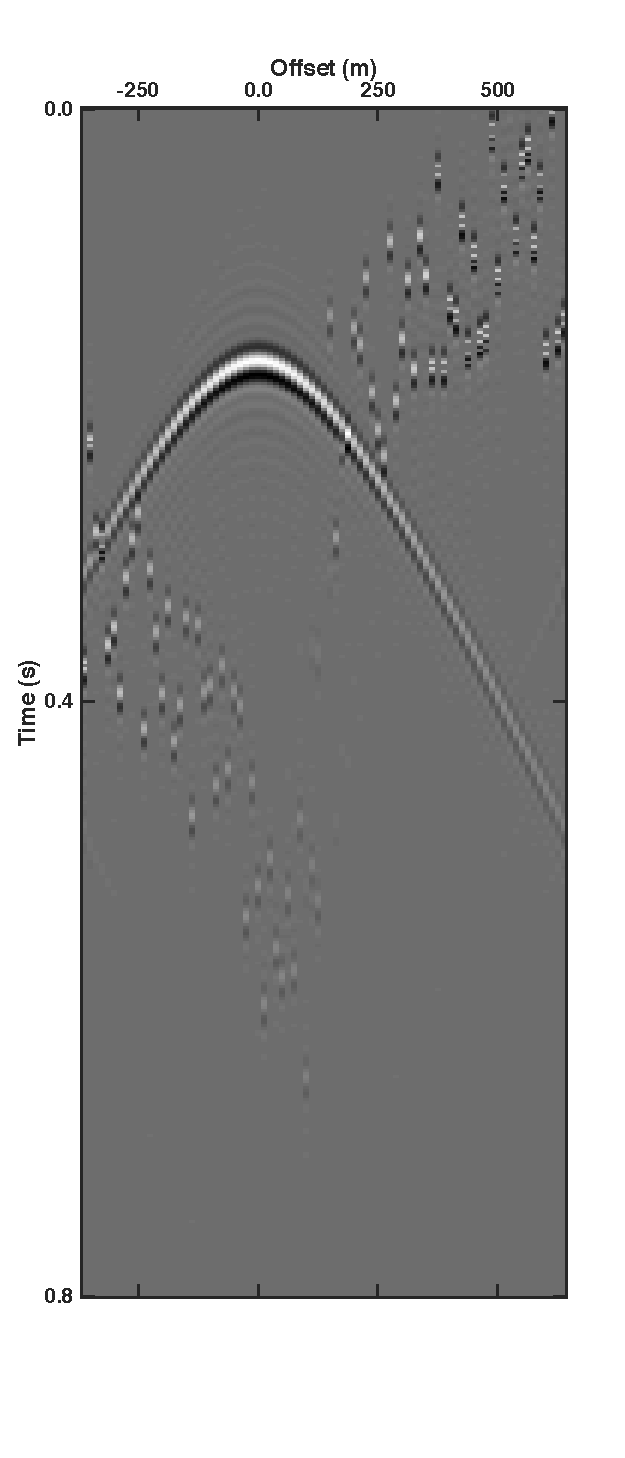
\includegraphics[width=\textwidth]{Plots/Mahdad/5iter/DeblendedCRG_rec30}	
		\caption{}
		\label{fig:Ch-Theory-Deblended}
	\end{subfigure}
	\caption{(a) Pseudo-deblended receiver gather. The subfigures (b)-(f) illustrate each step of the deblending algorithm. For better visibility examples from the $5^{th}$ iteration are chosen. (b) $f$-$k$-spectrum before (top) and after (bottom) $f$-$k$-filtering, (c) $f$-$k$-filtered common receiver gather, (d) after thresholding, (e) estimated source interference (f) estimated data.}
	\label{fig:Ch-Theory-IterativeDeblending}
\end{figure}

\begin{figure}
	\centering
	\begin{subfigure}[t]{0.25\textwidth}
		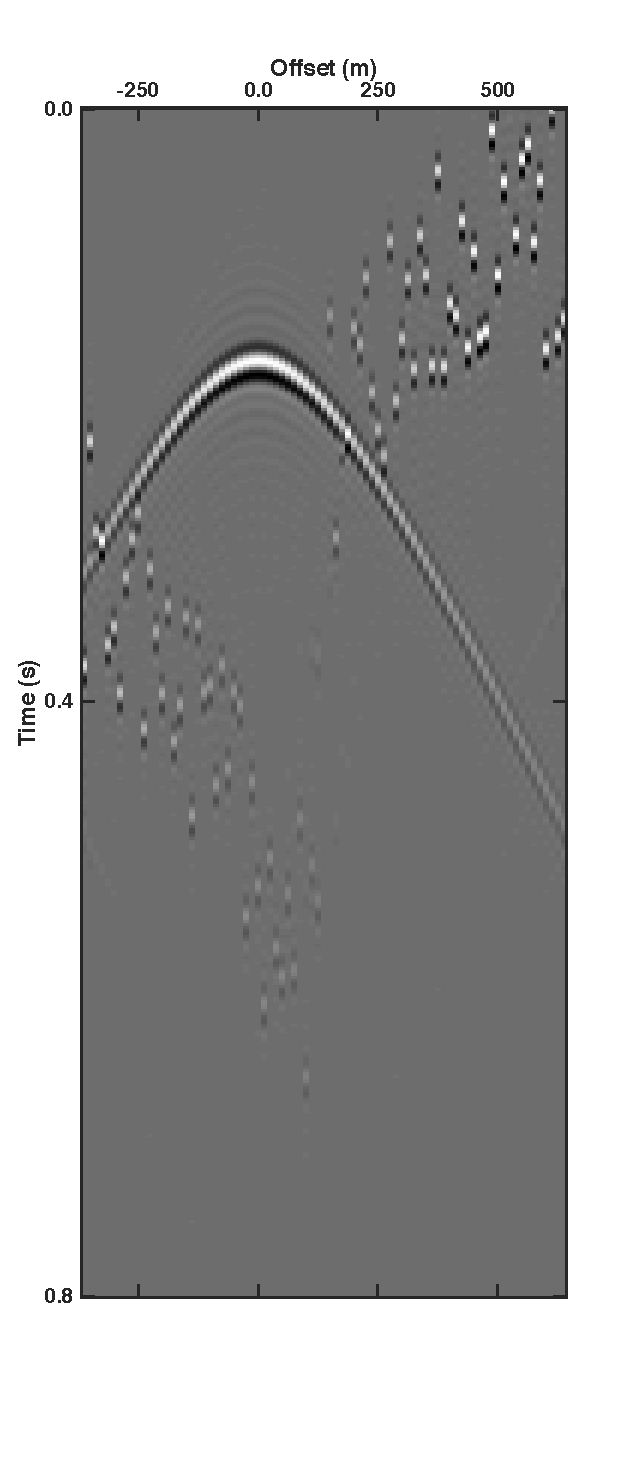
\includegraphics[width=\textwidth]{Plots/Mahdad/1iter/DeblendedCRG_rec30}	
		\caption{1 Iteration}
		\label{fig:Ch-Theory-DeblendedCRG1}
	\end{subfigure}
	%
	\centering
	\begin{subfigure}[t]{0.25\textwidth}
		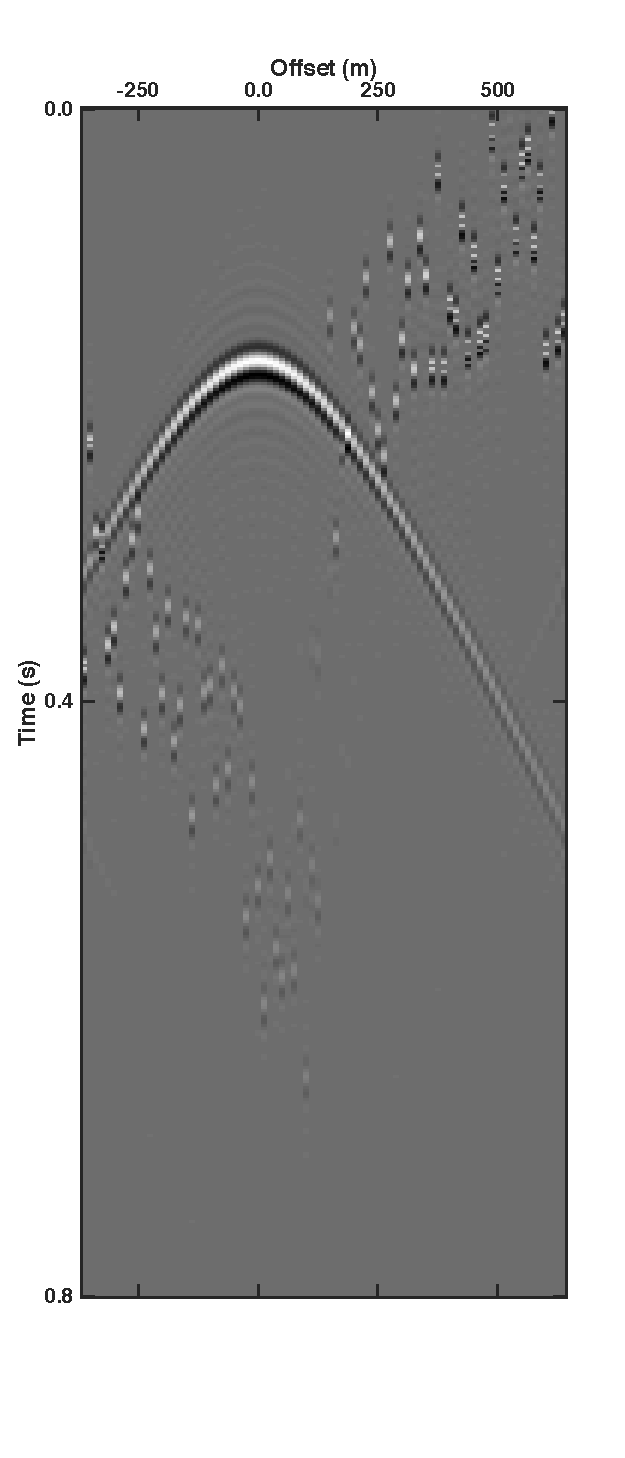
\includegraphics[width=\textwidth]{Plots/Mahdad/5iter/DeblendedCRG_rec30}	
		\caption{5 Iterations}
		\label{fig:Ch-Theory-DeblendedCRG5}
	\end{subfigure}
	%
	\begin{subfigure}[t]{0.25\textwidth}
		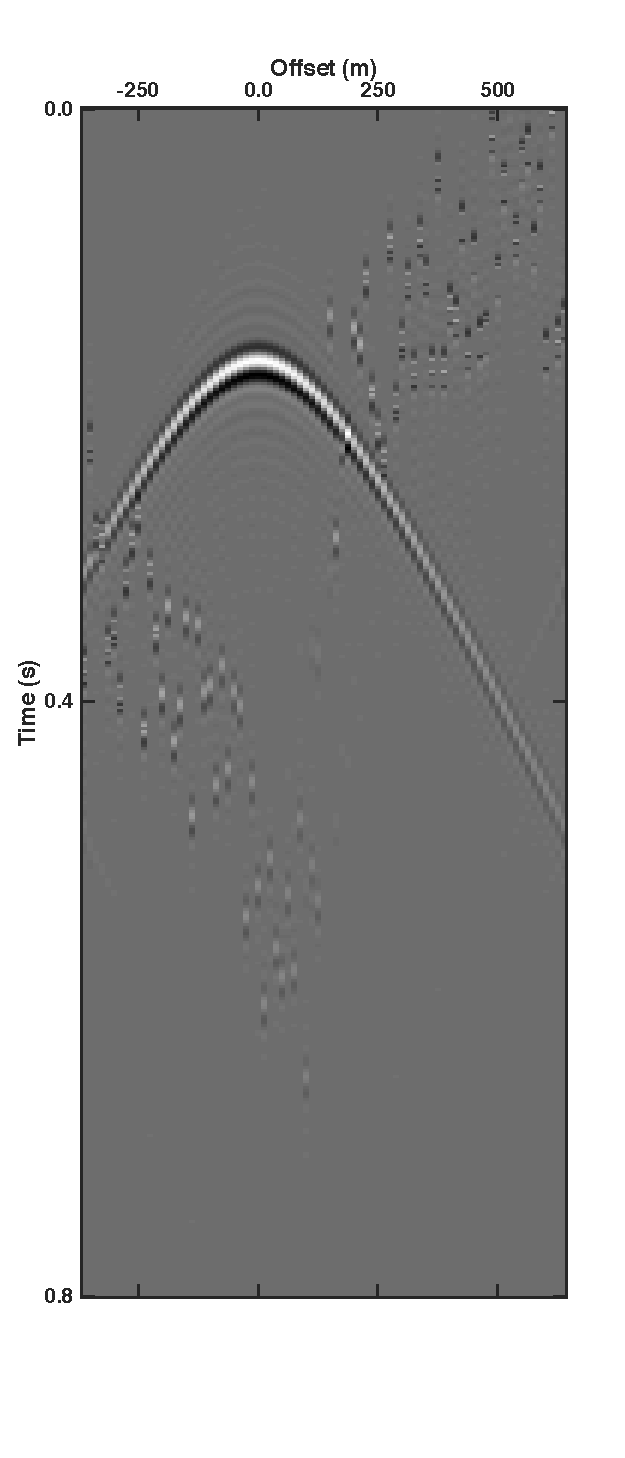
\includegraphics[width=\textwidth]{Plots/Mahdad/10iter/DeblendedCRG_rec30}	
		\caption{10 Iterations}
		\label{fig:Ch-Theory-DeblendedCRG10}
	\end{subfigure}
	%
	\begin{subfigure}[t]{0.25\textwidth}
		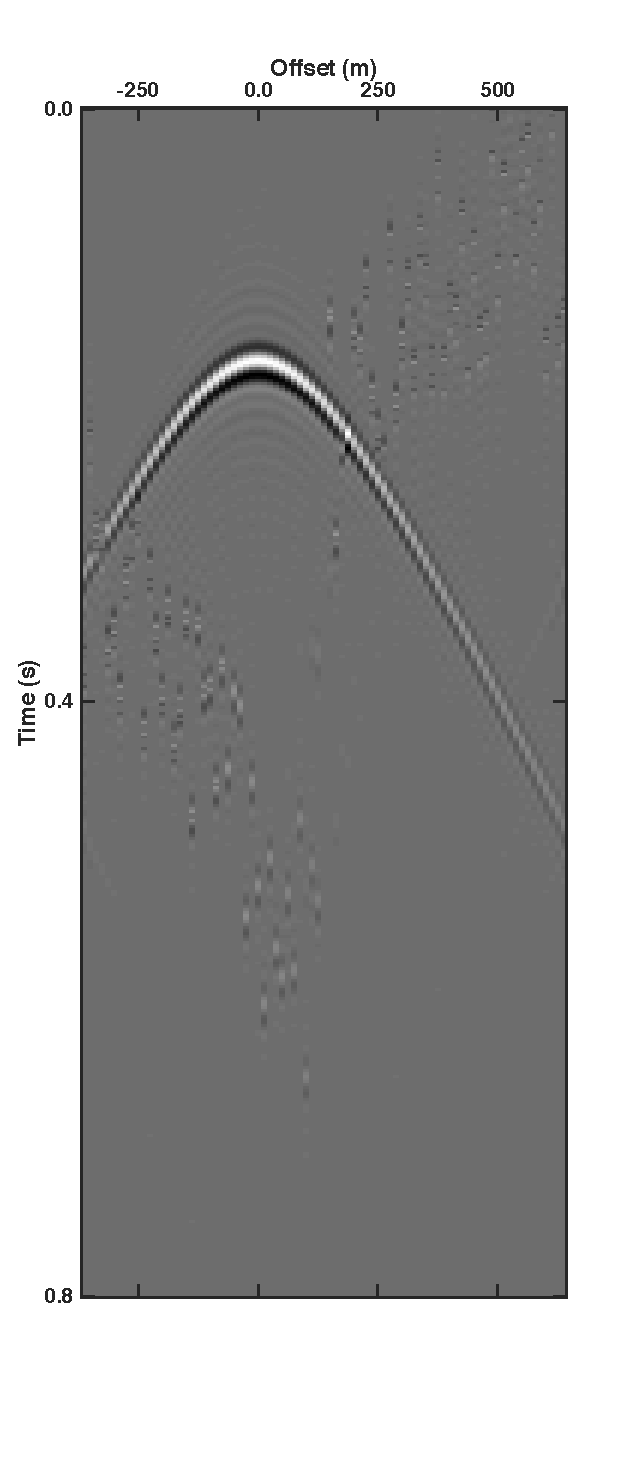
\includegraphics[width=\textwidth]{Plots/Mahdad/15iter/DeblendedCRG_rec30}	
		\caption{15 Iterations}
		\label{fig:Ch-Theory-DeblendedCRG15}
	\end{subfigure}
	%
	\begin{subfigure}[t]{0.25\textwidth}
		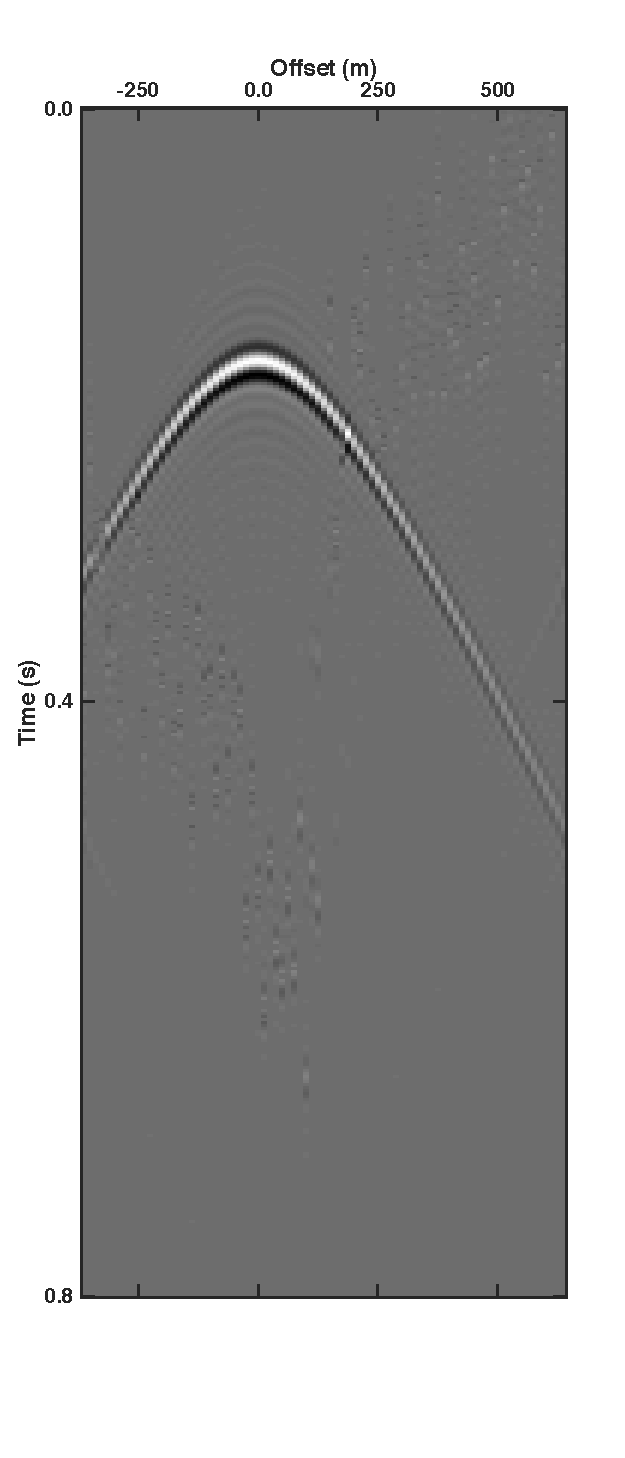
\includegraphics[width=\textwidth]{Plots/Mahdad/20iter/DeblendedCRG_rec30}	
		\caption{20 Iterations}
		\label{fig:Ch-Theory-DeblendedCRG20}
	\end{subfigure}
	%
	\begin{subfigure}[t]{0.25\textwidth}
		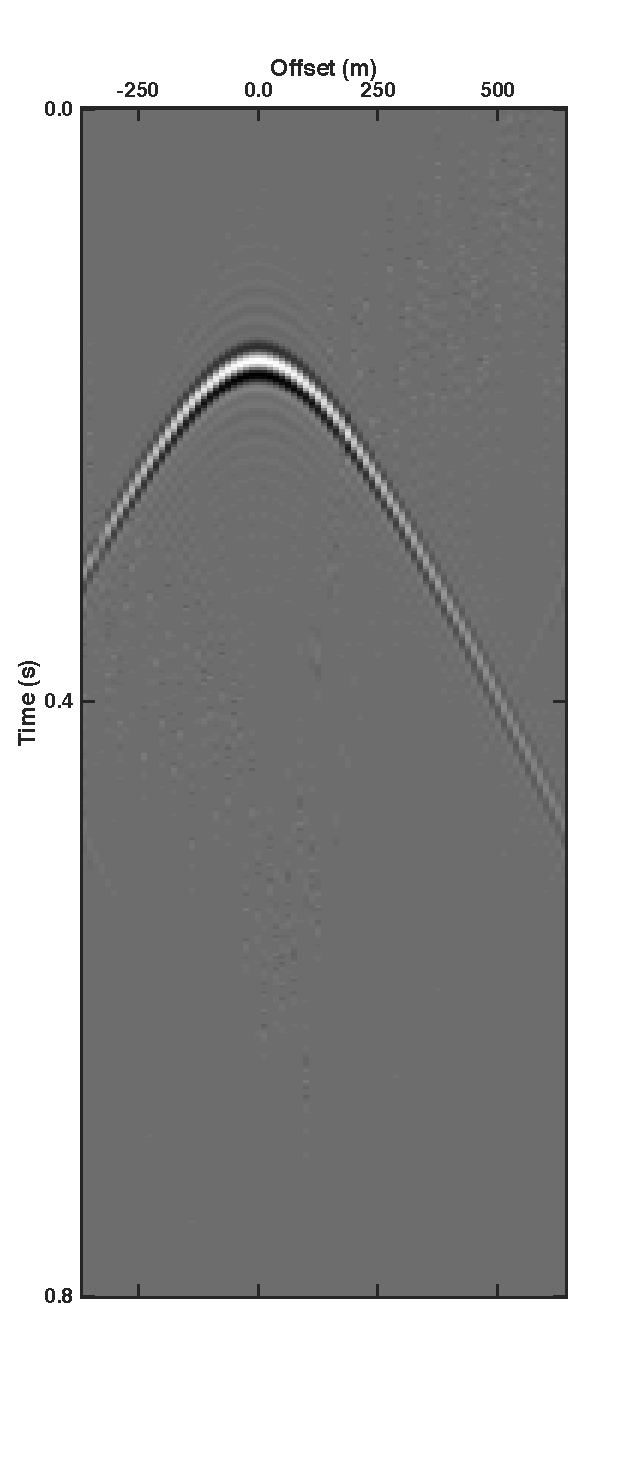
\includegraphics[width=\textwidth]{Plots/Mahdad/25iter/DeblendedCRG_rec30}	
		\caption{25 Iterations}
		\label{fig:Ch-Theory-DeblendedCRG25}
	\end{subfigure}
	\caption{Common receiver gather of the estimated data after 1, 5, 10, 15, 20 and 25 iterations.}
	\label{fig:Ch-Theory-EstimatedData}

\end{figure}



\subsubsection*{Thresholding}
The second constraint for the estimation of the unblended data is sparsity in the space time domain.

After $f$-$k$-filtering the spiky noise is attenuated (see Figure \ref{fig:Ch-Theory-FKFiltered}). Next, one defines a threshold in the $x$-$t$ domain, which is larger than the noise amplitudes and smaller than the highest signal amplitudes. Only amplitudes above the threshold are picked, i.e. only signal with strong amplitudes is selected (see Figure \ref{fig:Ch-Theory-Threshold}). 

The resulting thresholded data, \textbf{\={P}}, is used to predict the source interference;

\begin{equation}
	\textbf{\^{N}}_\textbf{i} = \textbf{\={P}} \, (\mathbf{\Gamma \, \Gamma^H} - \textbf{I}),
	\label{eq:Ch-Theory-NoiseEstimation}
\end{equation}

which is illustrated in Figure \ref{fig:Ch-Theory-Noise}.

At each iteration the blending noise is attenuated further, such that the threshold can be lowered. Hence, the predicted source interference increases and approaches the true source interference. 

Thresholding allows to reduce aliased frequency components of the blending noise. Thus, the combination of $f$-$k$-filtering and thresholding is very powerful.

\subsubsection*{Blending Noise Subtraction} 
The estimate of the unblended data matrix \textbf{\^{P}}$_\textbf{i}$ is updated by subtracting the noise from the pseudo-deblended data,

\begin{equation}
	\textbf{\^P}_\textbf{i+1} = \textbf{P}_\textbf{bl} \, \mathbf{\Gamma^H} - \textbf{\^{N}}_\textbf{i}, 
	\label{eq:Ch-Theory-DataUpdate1}
\end{equation}

which is shown in Figure \ref{fig:Ch-Theory-Deblended}.

This process is repeated iteratively till convergence is reached. In this context convergence can be defined as the point where the difference $\mid \textbf{\^P}_\textbf{i+1} - \textbf{\^{P}}_\textbf{i} \mid$ drops below a predefined limit. Alternatively, one can set a maximum number of iterations. 

Figure \ref{fig:Ch-Theory-EstimatedData} shows the estimate of the unblended data for increasing iterations. One can observe that the blended shot is successively  attenuated.



\section{Analysis of the Blending Matrix} \label{sec:BlendingMatrix}

In order to optimize the blended acquisition design, one must understand the properties of the blending matrix $\mathbf{\Gamma}$ and its influence on the deblending performance.

The blending matrix $\mathbf{\Gamma}$ determines the pseudo-deblended data,

\begin{equation}
	\mathbf{ P_{ps} } = \mathbf{P \Gamma \Gamma ^H},
	\label{eq:Ch-Theory-Pseudo-Deblended-Data}
\end{equation}

which is a superposition of the unblended data, $\mathbf{P}$, and the source interference, $\mathbf{N}$,

\begin{equation}
	\mathbf{P_{ps}} = \mathbf{P} + \mathbf{N}.
	\label{eq:Ch-Theory-PseudoSuperposition}
\end{equation}

The more incoherent the source interference, $\mathbf{N}$, the better it can be removed by noise filters.

In the following the effect of the blending matrix, $\mathbf{\Gamma}$, on the product $\mathbf{\Gamma \Gamma^H}$ and on the pseudo-deblended data is analyzed. For simplicity, it is assumed that the blending matrix, $\mathbf{\Gamma}$, only contains phase shift terms, $\mathrm{e}^{-j \omega \Delta t}$, with an amplitude equal to 1 or 0. It is also assumed that each source is fired only once, unlike the shot repetition case \citep{Sixue}.

Each row of $\mathbf{\Gamma}$ represents a source $k$ and each column of $\mathbf{\Gamma ^H}$ represents a source $l$ with a complex conjugated phase term (see Figure \ref{fig:Ch-Theory-GGH}). Hence, each element $g_{kl}$ of the matrix $\mathbf{\Gamma \Gamma^H}$ is the dot product between the $k^{th}$ source and the complex conjugate of the $l^{th}$ source.

\begin{figure}
	\centering
	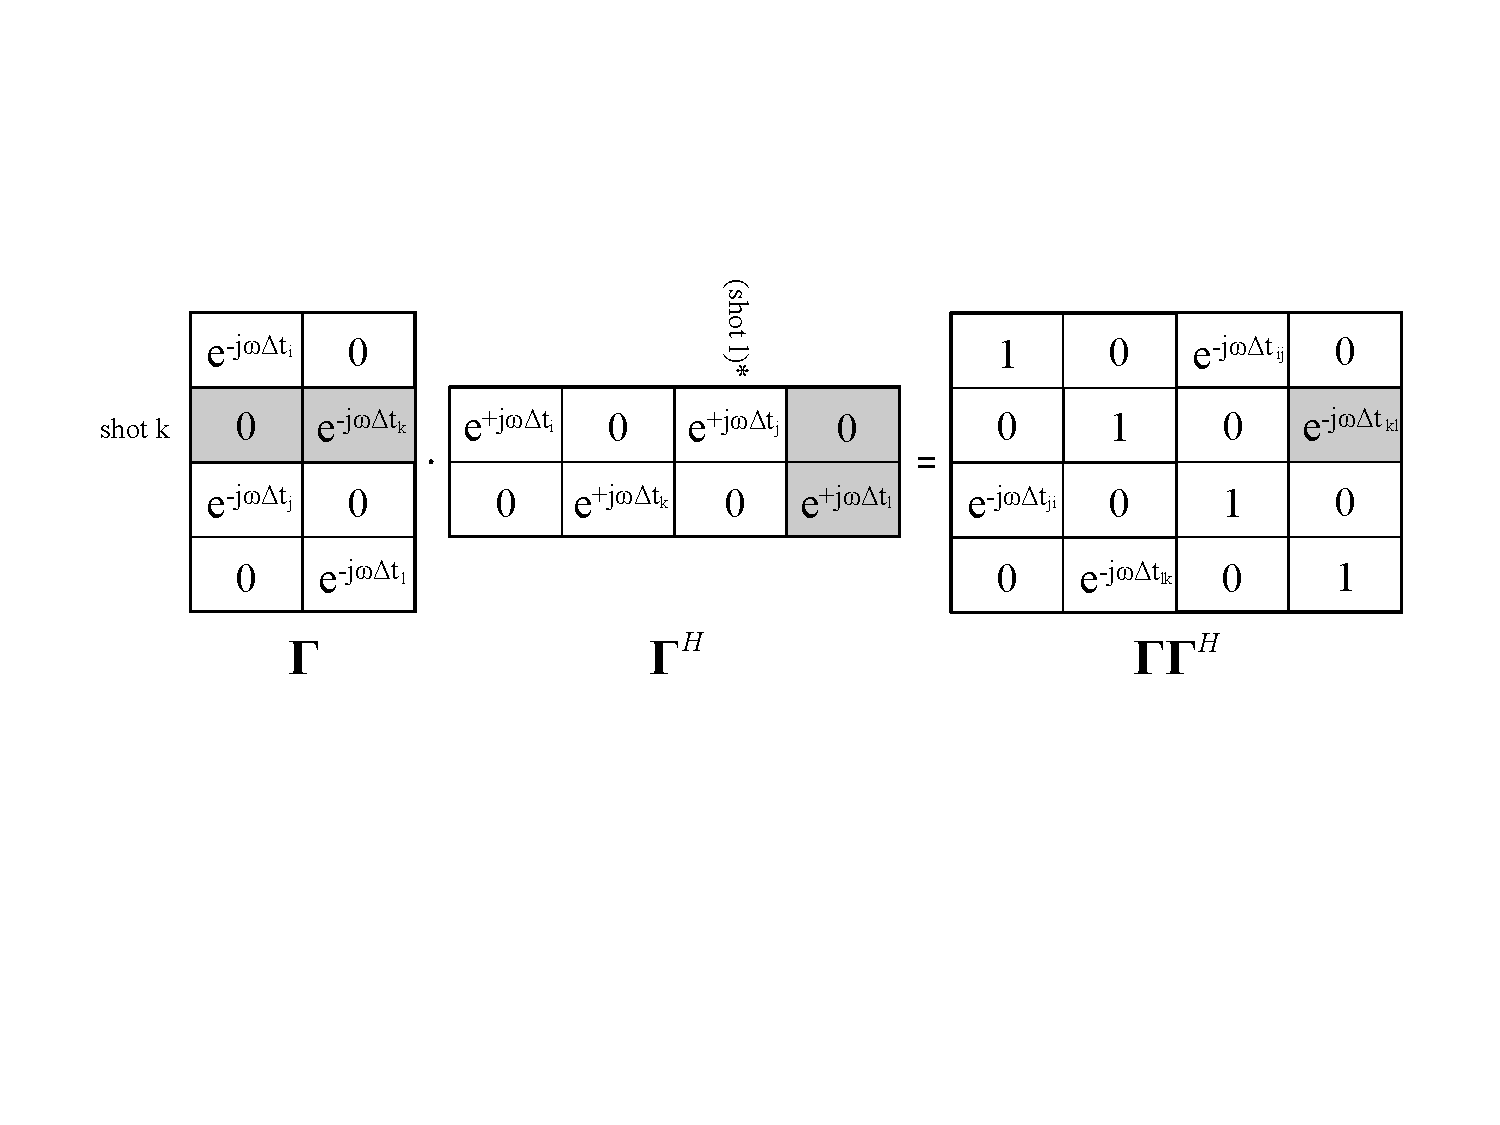
\includegraphics[width = \textwidth]{Plots/GGH}
	\caption{Illustration of the matrix product, $\mathbf{\Gamma \Gamma^H}$. In this notation $\Delta t_k$ refers to the phase shift of the source $k$, and $\Delta t_{kl}$ refers to the phase shift between the sources $k$ and $l$, $\Delta t_{kl} = \Delta t_k - \Delta t_l$.}
	\label{fig:Ch-Theory-GGH}
\end{figure}

Consequently, an element $g_{kl}$ of the product $\mathbf{\Gamma \Gamma ^H}$ represents the overlap of the sources $k$ and $l$ for all experiments. The main diagonal of $\mathbf{\Gamma \Gamma ^H}$ refers to the overlap of each source with itself, which of course is perfect and therefore equal to 1. The off diagonal elements of $\mathbf{\Gamma \Gamma ^H}$ are either 0 if the associated sources do not overlap, or contain a phase shift, $\mathrm{e}^{\, -j \omega \Delta t_{kl}}$.

In equation \ref{eq:Ch-Theory-Pseudo-Deblended-Data} the main diagonal elements of $\mathbf{\Gamma \Gamma ^H}$ copy the data matrix, $\mathbf{P}$, while the off-diagonal elements create the source interference, $\mathbf{N}$. If the elements $g_{ik}$ along a sub-diagonal are in phase, they will shift the columns of the data matrix and apply a coherent phase shift to each of them (see Figure \ref{fig:Ch-Theory-PseudoCRG-CoherentDelay}). Instead if the elements $g_{ik}$ along a sub-diagonal are out of phase, they will shift the columns of the data matrix and distort the phase of each column (see Figure \ref{fig:Ch-Theory-PseudoCRG-IncoherentDelay}). 

Figure \ref{fig:Ch-Theory-PseudoCRG-FK-CoherentDelay} and \ref{fig:Ch-Theory-PseudoCRG-FK-IncoherentDelay} display the $f$-$k$-spectra of the pseudo-blended data for constant and random firing time delays respectively. In the case of constant firing time delays almost all of the energy maps in the signal cone. In the case of random firing time delays a significant part of the energy maps outside of the signal cone. Therefore, the coherency constraint performs better for random firing delays.  

\begin{figure}
	\centering
	\begin{subfigure}[b]{0.3\textwidth}
		\centering
		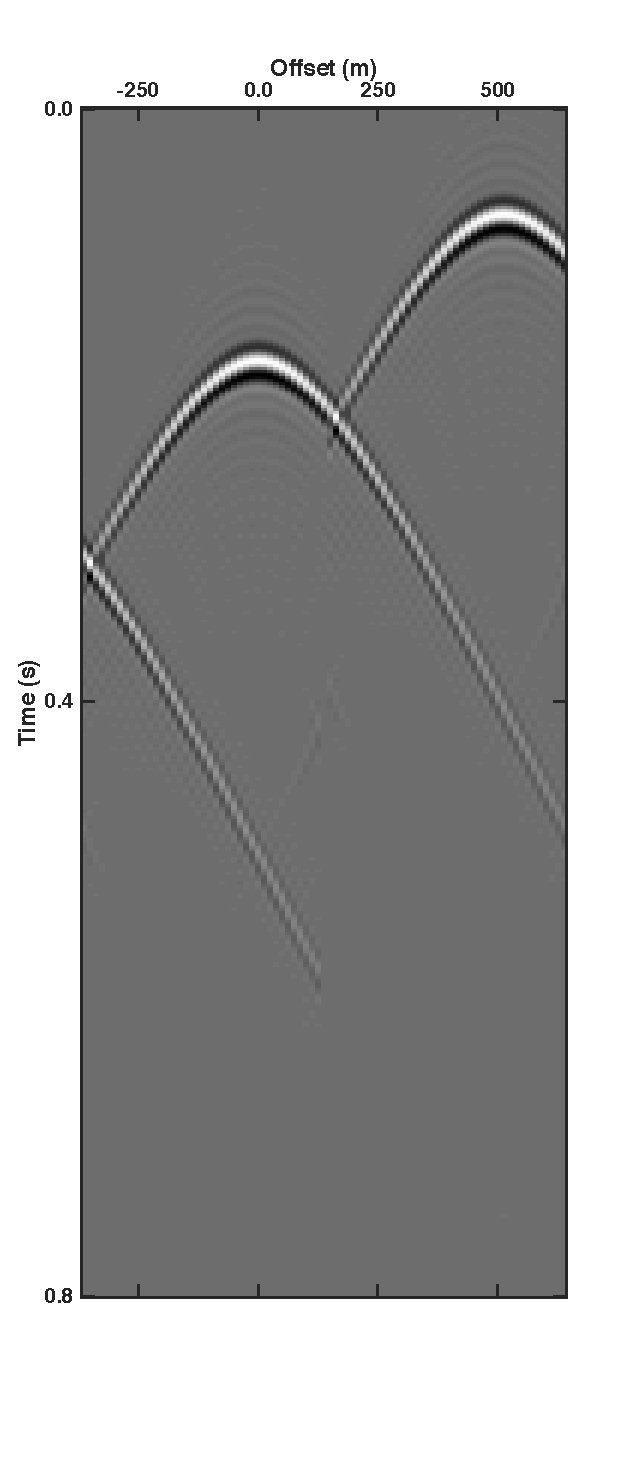
\includegraphics[width = \textwidth]{Plots/Mahdad/25iter/TimeDelay/Pseudo-DeblendedCRG_rec30_coh}
		\caption{}
		\label{fig:Ch-Theory-PseudoCRG-CoherentDelay}
	\end{subfigure}
	%
	\centering
	\begin{subfigure}[b]{0.3\textwidth}
		\centering
		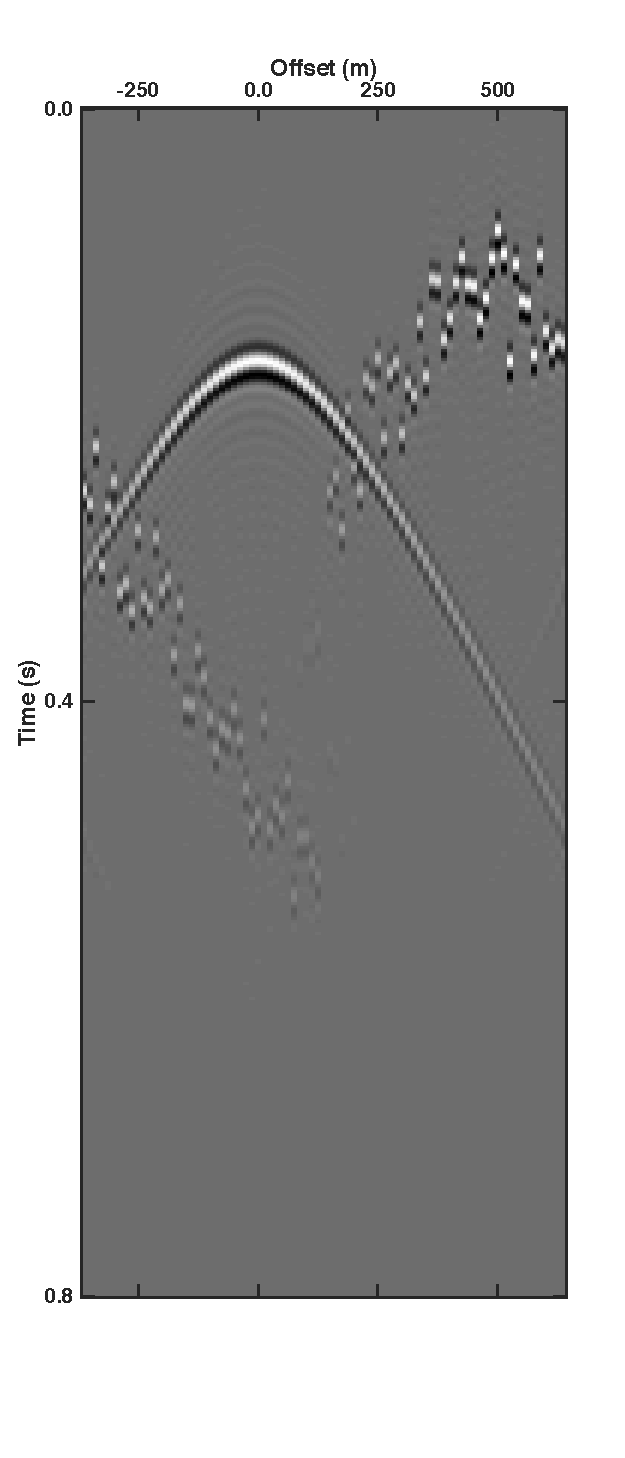
\includegraphics[width = \textwidth]{Plots/Mahdad/25iter/TimeDelay/Pseudo-DeblendedCRG_rec30}
		\caption{}
		\label{fig:Ch-Theory-PseudoCRG-IncoherentDelay}
	\end{subfigure}
	%
	\centering
	\begin{subfigure}[b]{0.3\textwidth}
	
		\centering
		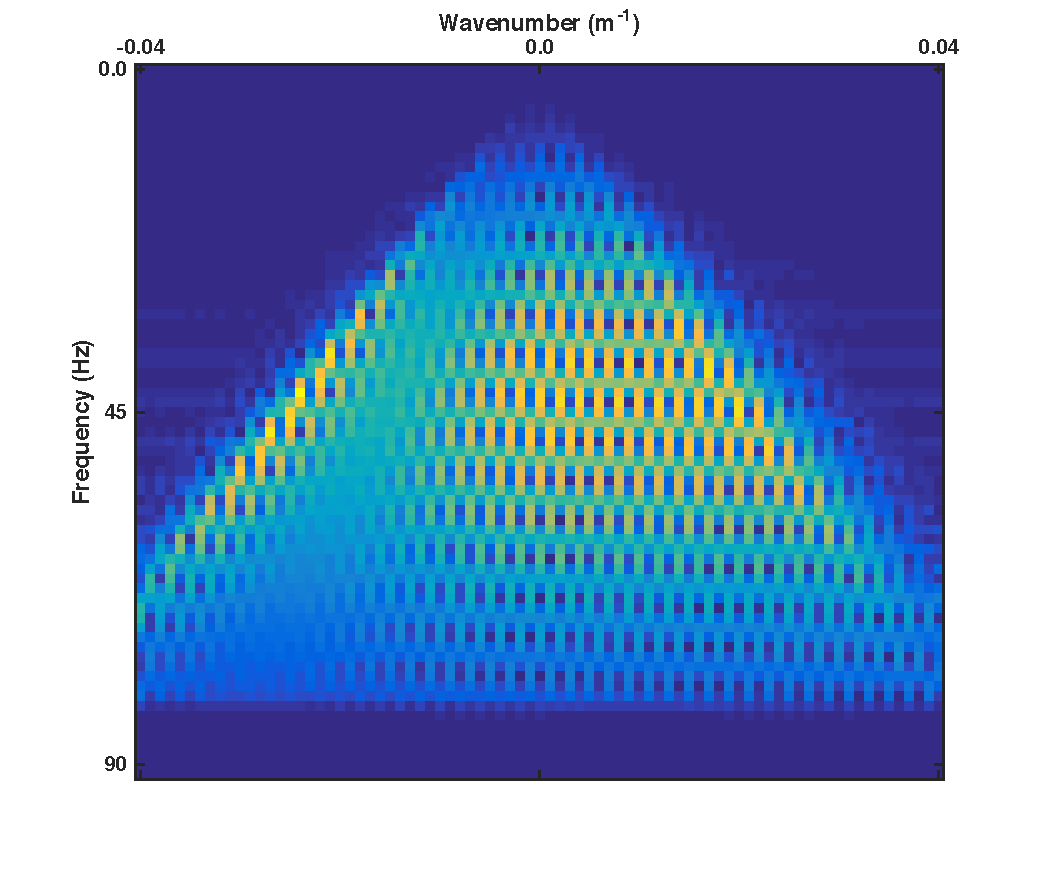
\includegraphics[width = \textwidth]{Plots/Mahdad/25iter/TimeDelay/FK-Pseudo-deblendedCRG_rec30_coh}
		\caption{}
		\label{fig:Ch-Theory-PseudoCRG-FK-CoherentDelay}
		
		\par\bigskip
		
		\centering
		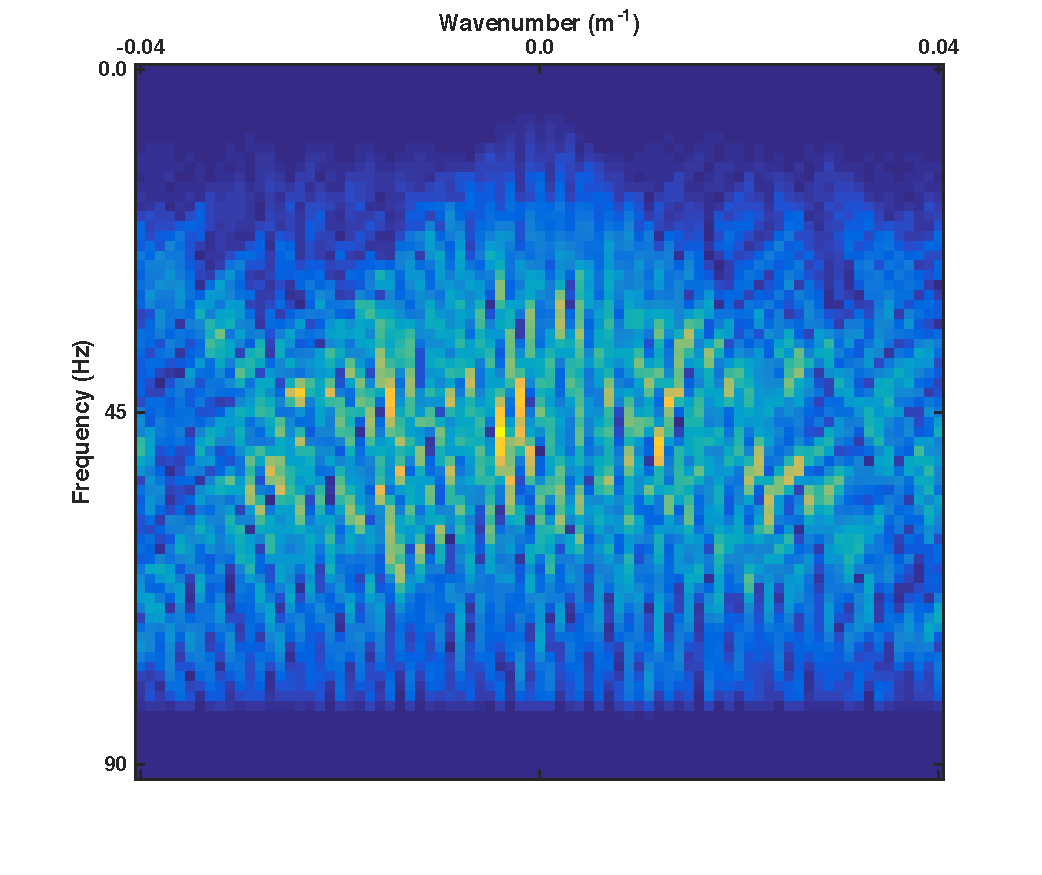
\includegraphics[width = \textwidth]{Plots/Mahdad/25iter/TimeDelay/FK-Pseudo-deblendedCRG_rec30}
		\caption{}
		\label{fig:Ch-Theory-PseudoCRG-FK-IncoherentDelay}
		
	\end{subfigure}
	
	\caption{Comparison of the pseudo-deblended receiver gather for (a) constant firing time delays of \SI{100}{\milli\second}, and (b) random firing time delays between \SI{0}{\milli\second} and \SI{100}{\milli\second}. (c) and (d) show the $f$-$k$-spectra of (a) and (b) respectively.}
	\label{fig:Ch-Theory-PseudoCRG-IncoherencyEffect}

\end{figure}

\begin{comment}
In order to generate incoherent source interference, $\mathbf{N}$, it is therefore favorable if the elements $a_{ik}$ of each lower or upper diagonal are out of phase. For example, considering the $n^{th}$ upper or lower diagonal of the matrix $\mathbf{\Gamma \Gamma^H}$ this observation translates to the acquisition as follows: All source pairs, which are $n$ sources apart from each other, must be fired incoherently. The incoherent firing is realized by delaying blended sources with a random time delay.
\end{comment}

Intuitively, the degree of incoherency of the source interference, $\mathbf{N}$, also depends on whether the sources blended in an experiment are selected randomly, or in a spatially coherent pattern. For example, one expects the source interference to be more incoherent if in each experiment randomly picked sources are blended, than if in each experiment adjacent sources are blended.

\todo[inline]{This might need some extra explanation and plot!}

\begin{comment}

In terms of the blending matrix $\mathbf{\Gamma}$ a spatially incoherent firing pattern means that the rows, i.e. the sources, are shuffled randomly. As a consequence the off-diagonal elements of the matrix product $\mathbf{\Gamma \Gamma^H}$ are reordered randomly. This shuffling process can help to further distort the phase of the interfering sources. However, if the maximum allowed time delay between blended sources is aready large the spatially incoherent blending pattern will not increase the incoherency of the interfering sources.   

In practice, the maximum allowed firing time delay is limited by the available acquisition time. The spatial distribution of blended sources is constraint by the acquisition design.
	
\end{comment}


\FloatBarrier

\section{Extension to 3D} \label{sec:MahdadMethod3d}

This thesis suggests to blend crossline sources, i.e. in combination with the movement of the seismic vessel one effectively blends sources in 3D.

The deblending method of \citet{Mahdad-Deblending-Method} is designed for 2D blended data. In principle, each step of the method can be applied to 3D data as well. In this thesis I will extend the deblending method of \citet{Mahdad-Deblending-Method} to 3D and demonstrate its performance.

First, the data sorting will be modified such that the blended 3D data can be described using the same forward model as in section \ref{sec:Ch-Theory-Operator}. Second, the $f$-$k$-filter will be extended to remove noise in crossline and inline direction. The presented data sorting will allow to maintain all other steps of the deblending algorithm of \citet{Mahdad-Deblending-Method} unchanged.

\subsection{Data Sorting} \label{sec:Ch-Theory-3dExtension-DataSorting}

\subsubsection*{Data Matrix}

In 3D acquisition the sources and receivers are distributed on a 2D surface. Thus, their locations are defined by their crossline and inline positions, ($x$, $y$). Each data point which is measured by a source receiver pair at a specific time is therefore constraint by 5 coordinates: Time $t$, receiver crossline and inline position ($x_r$, $y_r$), and source crossline and inline position ($x_s$, $y_s$).

Before applying the Mahdad deblending method the 5D data array will be reorganized in a 2D data matrix according to \citet{Delphi-Format}. For this data sorting a 1D Fourier transform with respect to time is performed and a frequency slice is selected. This reduces the data array from 5 to 4 dimensions. 

The 4D data array is sorted in a 2D matrix data matrix, $\mathbf{P}$, with as many rows as receivers and as many columns as sources. The total number of receivers (or sources) is obtained by multiplying the number of crossline and inline receivers (or sources). Assume there are $Ns_x$ sources per crossline. The sources of the first crossline are assigned to the first $Ns_x$ columns of the data matrix, the sources of the second crossline are assigned to the next $Ns_x$ columns of the data matrix, etc. The cross- and inline receivers are sorted in the rows of the data matrix in analogy. This is illustrated in Figure \ref{fig:Ch-Theory-DelphiFormat} and \ref{fig:Ch-Theory-DataSorting}. 

\begin{figure}
	\centering
	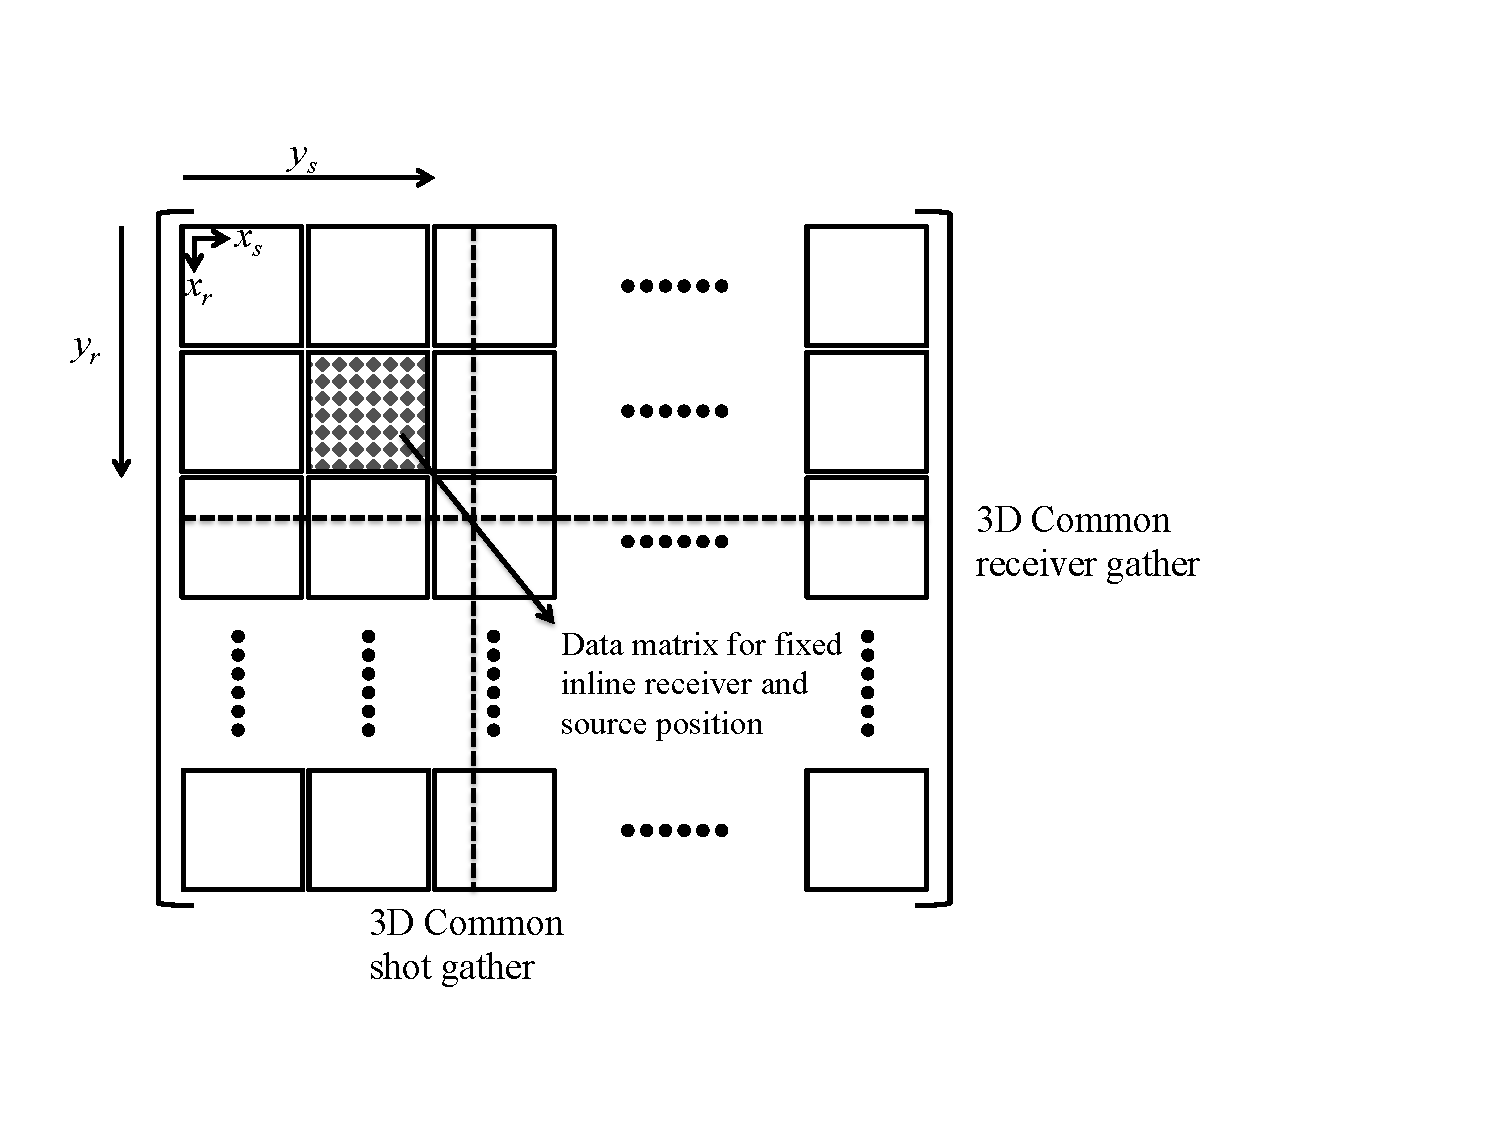
\includegraphics[width=0.6\textwidth]{Plots/DelphiFormat-v2}
	\caption{Illustration of the data matrix $\mathbf{P}$ for 3D data \citep{Delphi-Format}. $y_r$ and $y_s$ represent the inline receiver and source positions. $x_r$ and $x_s$ represent the crossline receiver and source positions. Each row refers to a 3D common receiver gather and each column to a 3D common shot gather. A sub-matrix with fixed receiver and source inline positions ($y_r$, $y_s$) is equivalent to a data matrix for 2D acquisition.}
	\label{fig:Ch-Theory-DelphiFormat}
\end{figure}


\begin{figure}
	
	\begin{subfigure}[t]{\textwidth}
	 	\centering
		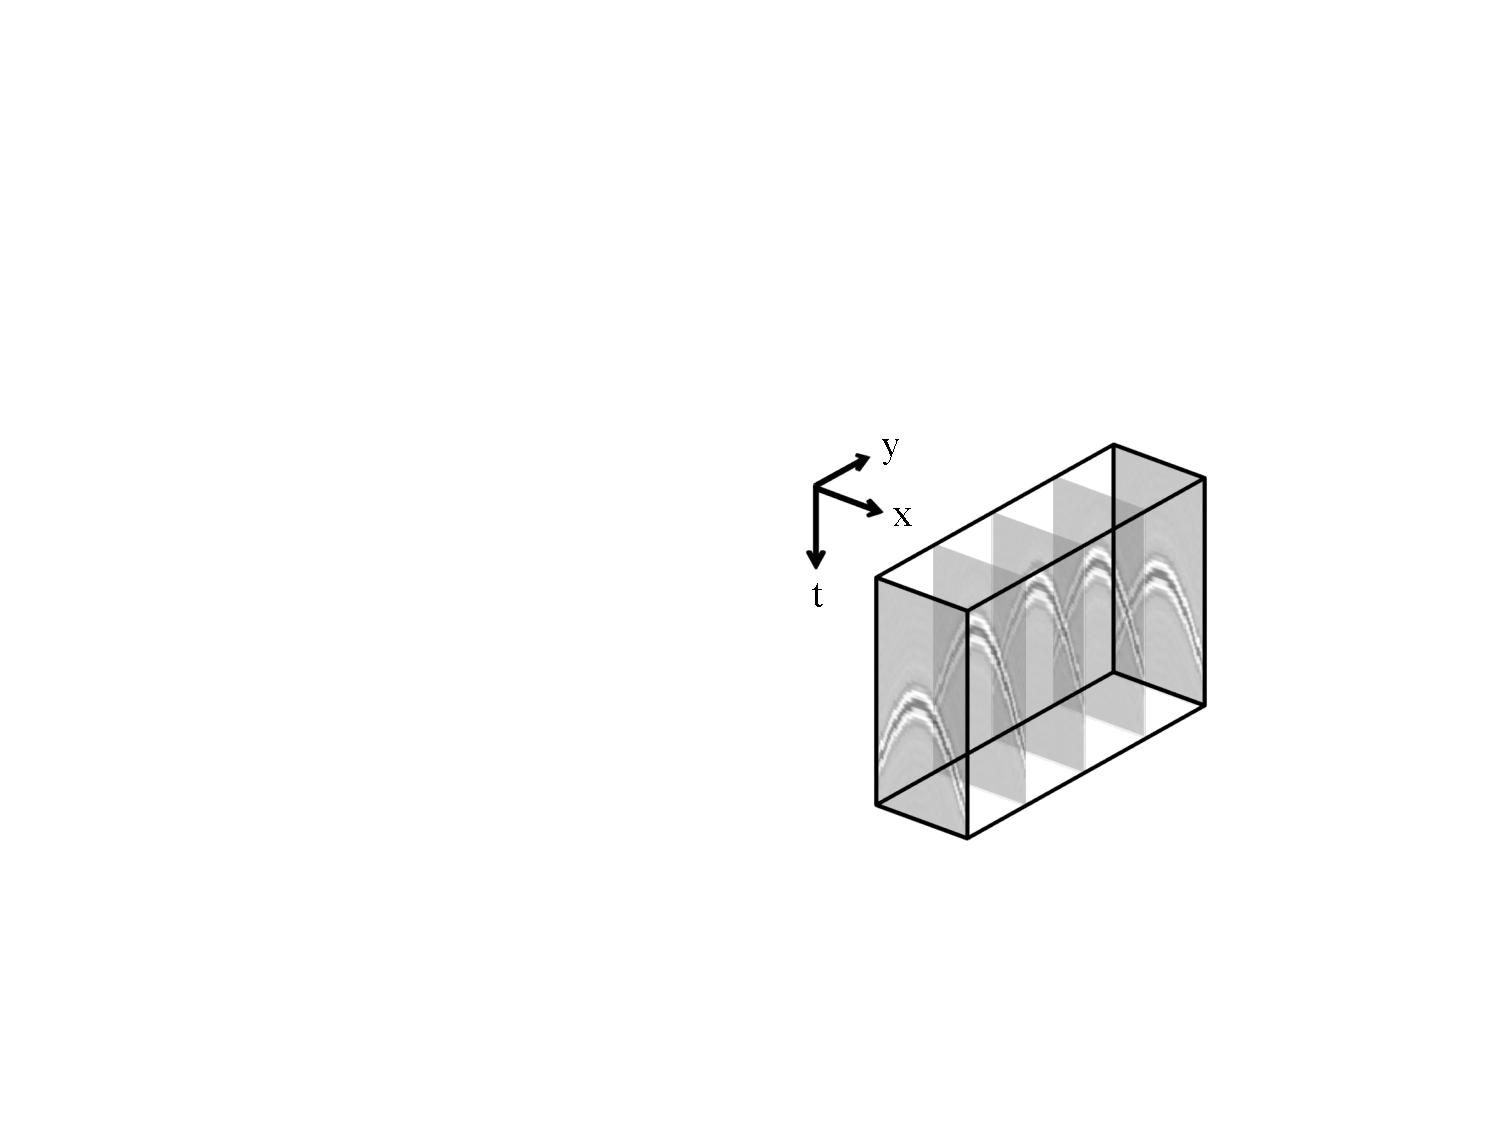
\includegraphics[width = 0.3\textwidth]{Plots/data3d}
		\caption{}
		\label{fig:Ch-Theory-Data3d}
	\end{subfigure}
	\par\bigskip
	\begin{subfigure}[t]{\textwidth}
		\centering
		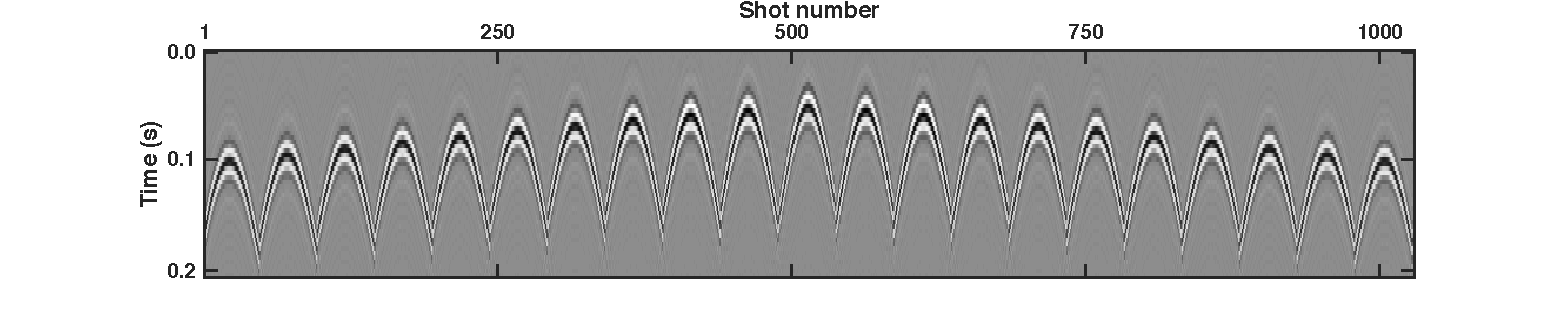
\includegraphics[width = \textwidth]{Plots/data3d_Delphi}
		\caption{}
		\label{fig:Ch-Theory-Data3d_Delphi}
	\end{subfigure}
	
	\caption{(a) Common receiver gather of a 3D data set with crossline (x) and inline (y) sources. (b) Resorted data set. Individual crossline sections are plotted next to each other in 2D.}
	\label{fig:Ch-Theory-DataSorting}
\end{figure}


\subsubsection*{Blending matrix}

As described in section \ref{sec:BlendingMatrix} each row of the blending matrix, $\mathbf{\Gamma}$, captures one source. For extension to 3D the sources of the first crossline are saved in the top $Ns_x$ rows of the blending matrix, followed by the sources of the second crossline etc. (see Figure \ref{fig:Ch-Theory-3D-BlendingMatrix-Design}). This framework allows to blend any source combination independent of the cross- and inline positions of the involved sources.

With the new data and blending matrix sorting one can already apply the 2D Mahdad method to the 3D data.

\begin{figure}

	\begin{subfigure}[t]{0.5\textwidth}
		\centering
		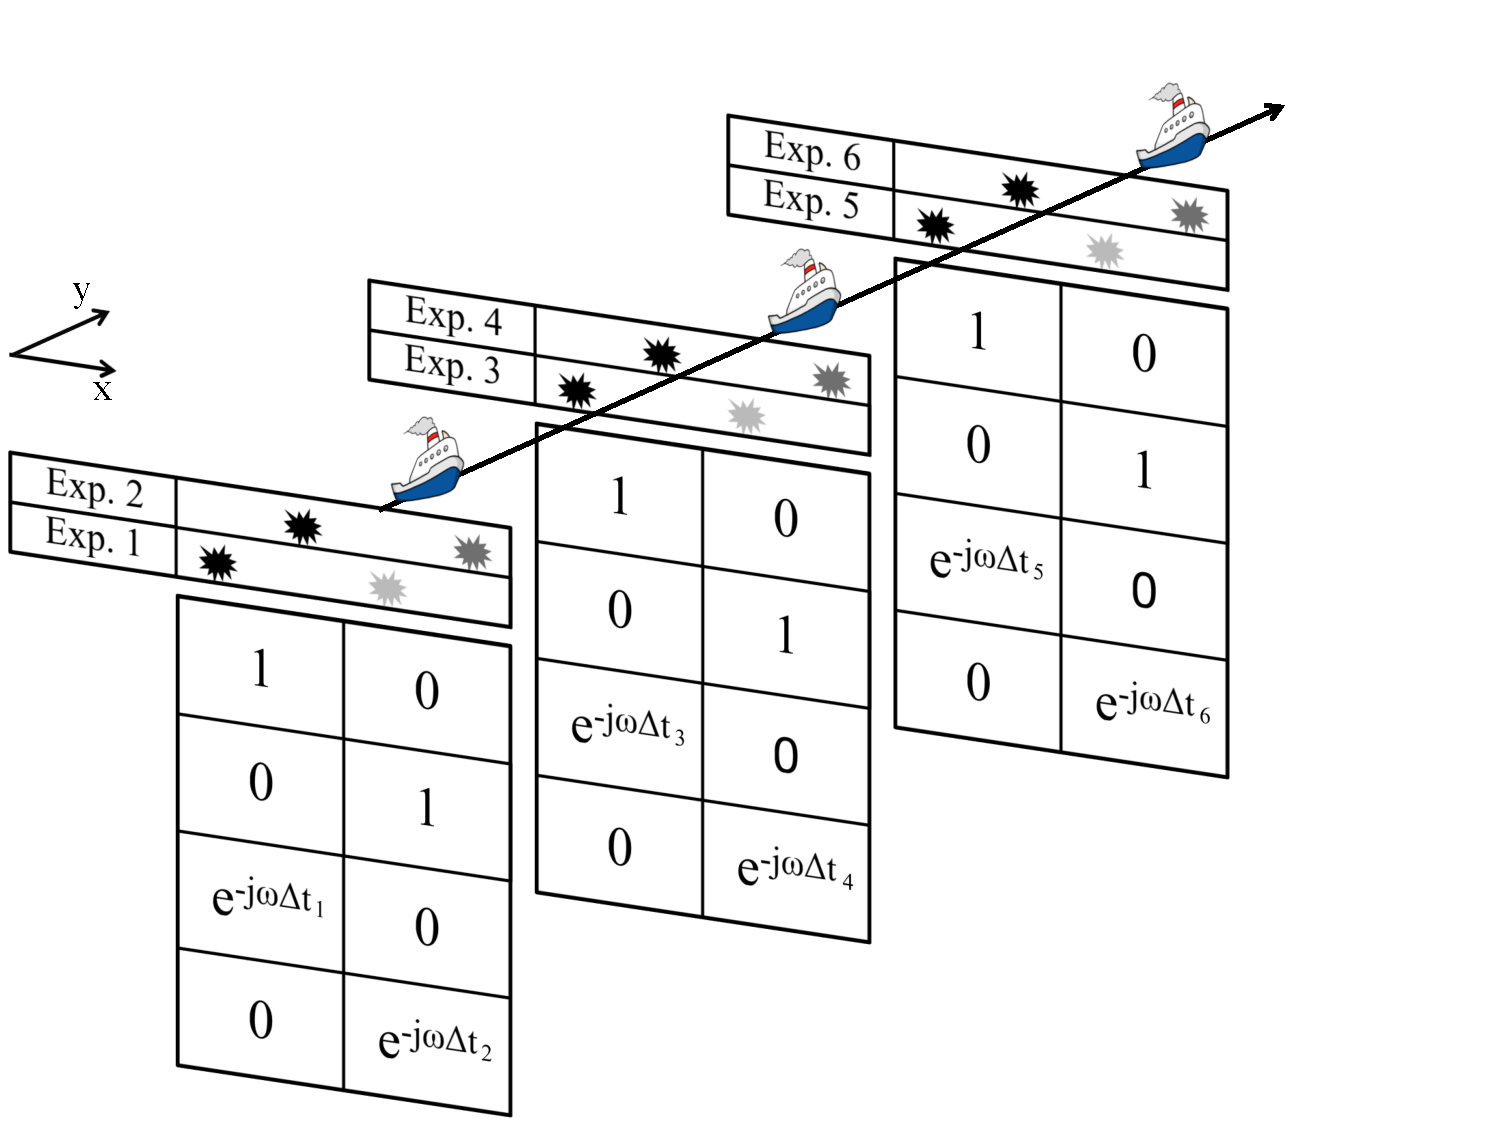
\includegraphics[width = \textwidth]{Plots/DrawingsCartesianFormat1}
		\caption{}
		\label{fig:Ch-Theory-3D-BlendedAcquisition}
	\end{subfigure}
	%
	\begin{subfigure}[t]{0.5\textwidth}
		\centering
		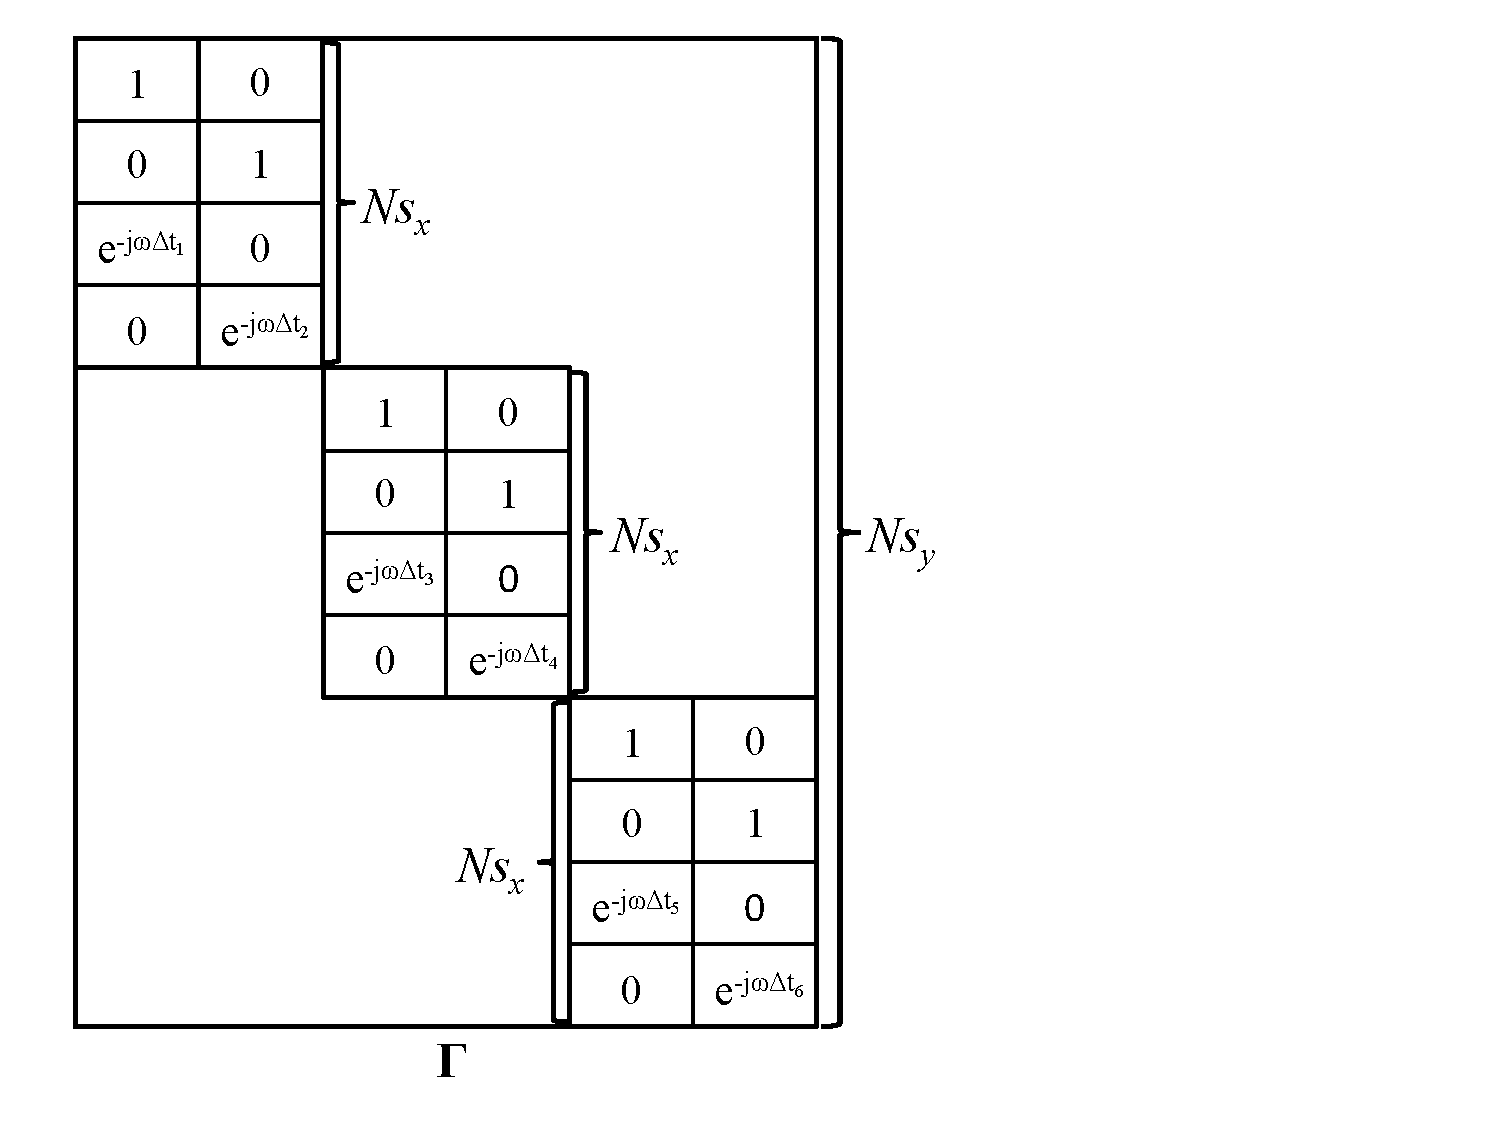
\includegraphics[width = 0.7\textwidth]{Plots/DrawingsCartesianFormat2}
		\caption{}
		\label{fig:Ch-Theory-3D-BlendingMatrix}
	\end{subfigure}
	
	\caption{Illustration of the blending matrix, $\mathbf{\Gamma}$, for 3D acquisition. (a) At each of the $Ns_y$ inline position the crossline sources ($x$ direction) are blended. Each of these 2D blending processes is described by a 2D blending matrix, which has as many rows as there are crossline sources, $Ns_x$. (b) The 2D blending matrices are assembled in a single 3D blending matrix, $\mathbf{\Gamma}$, which has $Ns_x$ by $Ns_y$ rows.}
	\label{fig:Ch-Theory-3D-BlendingMatrix-Design}

\end{figure}

\subsection{3D FKK Filter} \label{sec:Ch-Theory-3dExtension-FKK}

For a 2D $f$-$k$-spectrum the minimum (physical) velocity of the subsurface, $v_{min}$, determines the maximum unaliased wavenumber, $k_{max}$,  for a given frequency, $f$,

\begin{equation}
	k_{max} = \frac{f}{v_{min}}.
	\label{eq_Ch-Theory-MaxWavenmber}
\end{equation} 

For each frequency, $f$, wavenumbers above $k_{max}$ are removed which results in a 2D signal cone.

For 3D data one obtains the $f$-$k$-$k$-spectrum by applying a n-dimensional Fourier transform to the 5D data array. Next, as Mahdad's deblending method is applied to common receiver gathers one picks a single receiver, i.e constant cross- and inline receiver number. This leaves a 2D matrix, which captures the cross- and inline wavenumbers ($k_x$, $k_in$). Again the maximum wavenumber is determined by equation \ref{eq_Ch-Theory-MaxWavenmber}. The total wavenumber, $k_{T}$,

\begin{equation}
	k_{T} = \sqrt{k_x^2 + k_{in}^2},
	\label{eq:Ch-Theory-TotalWavenumber}
\end{equation}

must be smaller than the maximum wavenumber, $k_{max}$. Hence the signal "cone" is defined by a circle. This is repeated for each frequency component, such that the overall $f$-$k$-$k$-mask is a 3D cone. Finally, this mask is computed for each receiver gather.

Once the mask is built for a 5D data array it can either be applied to filter a 5D data array, or the mask is sorted to 2D according to section \ref{sec:Ch-Theory-3dExtension-DataSorting} and applied to the $f$-$k$-$k$-spectrum of the data matrix.

\todo[inline]{Show plots to illustrate the difference between fk and fkk mask. Maybe add a plot of the same data as in the part about 3d extension of the blending matrix but with a 3d fkk filter.}

















